%-------------------------------------------------------------------------------
%                            BAB IV
%               		HASIL DAN PEMBAHASAN
%-------------------------------------------------------------------------------
% \fancyhf{} 
% \fancyfoot[R]{\thepage}
\chapter{HASIL DAN PEMBAHASAN}
%\thispagestyle{plain} % Halaman pertama bab menggunakan gaya plain

\section{Pengumpulan Data}

\par Pengumpulan \textit{dataset} PathVQA dan VQA-RAD dilakukan melalui pengunduhan dari platform Huggingface menggunakan pustaka Huggingface Datasets versi 2.18.0. Sampel data dari kedua \textit{dataset} ini dapat dilihat pada Gambar \ref{fig:sample-data-pathvqa} dan Gambar \ref{fig:sample-data-vqarad}.

\begin{figure}[H]
  \centering
  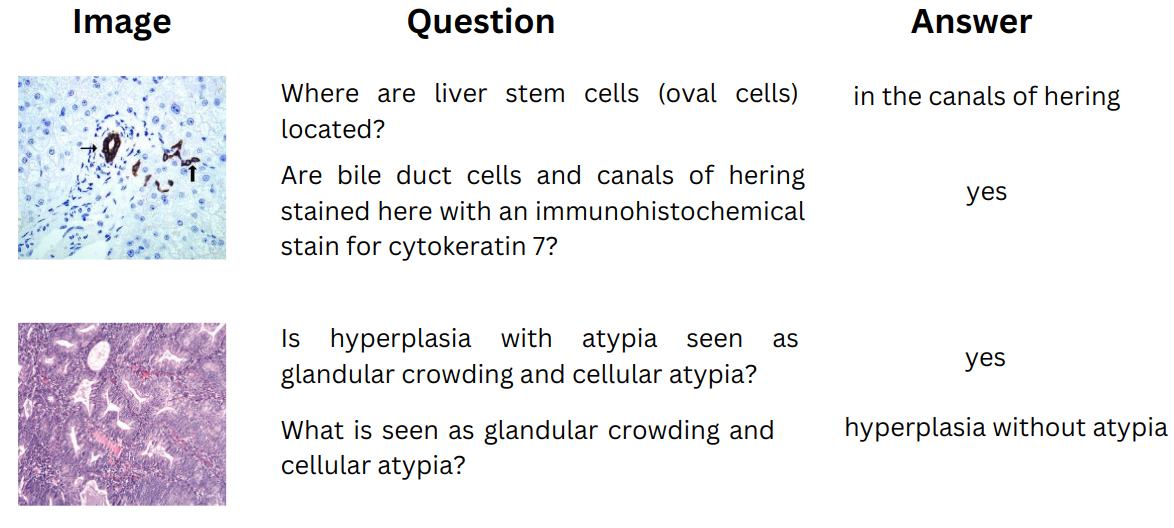
\includegraphics[width=14cm]{image/bab4/sample-pathvqa.png}
  \caption{Sampel data dari \textit{dataset} PathVQA}
  \label{fig:sample-data-pathvqa}
\end{figure}

\begin{figure}[H]
  \centering
  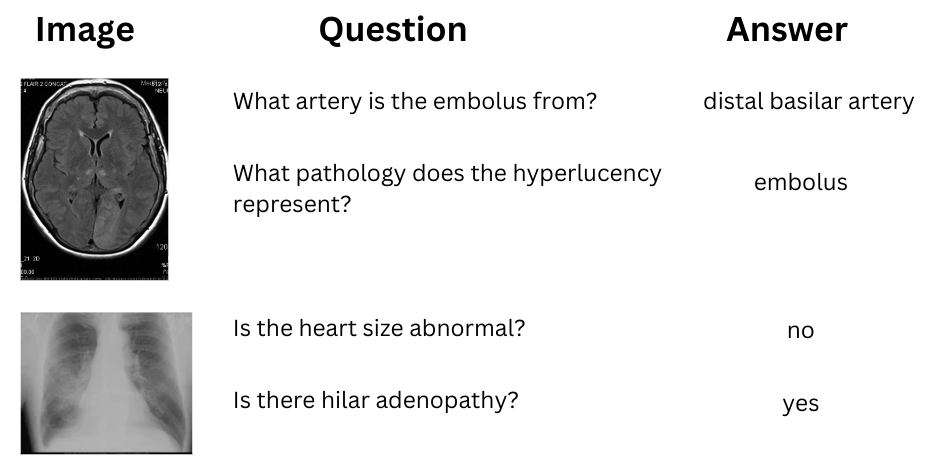
\includegraphics[width=14cm]{image/bab4/sample-vqarad.png}
  \caption{Sampel data dari \textit{dataset} VQA-RAD}
  \label{fig:sample-data-vqarad}
\end{figure}

Kedua \textit{dataset} ini memiliki struktur data bertipe \textit{DatasetDict}, yang merupakan format struktur data khas dari \textit{dataset} Huggingface. Dalam penelitian ini, kedua \textit{dataset} dikonversi menjadi format JSON (\textit{JavaScript Object Notation}) untuk memudahkan penulis dalam mengolah data gambar dan teks. Apabila menggunakan format \textit{DatasetDict}, penulis perlu mengakses data tersebut dengan menerapkan metode atau teknik tertentu sesuai dengan dokumentasi dari Huggingface. Konversi data ke format JSON memungkinkan penulis untuk mengakses dan melakukan pemrosesan data gambar dan teks sesuai dengan keinginan penulis.

\par Pada bagian pemrosesan gambar, penulis menemukan ada beberapa gambar di \textit{dataset} PathVQA yang memiliki format gambar selain \textit{Red Green Blue} (RGB), yaitu \textit{Cyan, Magenta, Yellow, Key (Black)} (CMYK). Pada bagian ini, penulis melakukan konversi gambar CMYK menjadi RGB menggunakan pustaka Python Imaging Library (PIL). Konversi gambar ini dilakukan untuk memastikan bahwa semua gambar dalam \textit{dataset} PathVQA memiliki format gambar yang sama, yaitu RGB. Pada gambar di \textit{dataset} VQA-RAD, semua gambar sudah memiliki format RGB, sehingga tidak perlu dilakukan konversi ke dalam bentuk RGB.

\par Pada bagian pemrosesan teks, kalimat dari pertanyaan telah dilakukan proses \textit{case folding}, \textit{remove punctuation}, \textit{stemming}, dan tokenisasi untuk menghasilkan kalimat yang lebih bersih dan lebih mudah diproses oleh model. 

\par Proses \textit{case folding} dilakukan untuk mengubah seluruh huruf dalam kalimat menjadi huruf kecil, sehingga model dapat memahami kata yang sama dengan huruf besar dan huruf kecil sebagai kata yang sama. Pada Tabel \ref{tab:sample-preprocessing-text-case-folding} terdapat contoh hasil dari proses \textit{case folding}. 

% Please add the following required packages to your document preamble:
% \usepackage{longtable}
% Note: It may be necessary to compile the document several times to get a multi-page table to line up properly
\begin{longtable}[c]{|l|l|}
  \caption{Proses \textit{case folding} pada sampel \textit{dataset} PathVQA dan VQA-RAD}
  \label{tab:sample-preprocessing-text-case-folding}\\
  \hline
  \textbf{Sebelum} &
    \textbf{Sesudah} \\ \hline
  \endfirsthead
  %
  \endhead
  %
  \textit{\begin{tabular}[c]{@{}l@{}}Where are liver stem cells\\  (oval cells) located?\end{tabular}} &
    \textit{\begin{tabular}[c]{@{}l@{}}where are liver stem cells\\  (oval cells) located?\end{tabular}} \\ \hline
  \textit{\begin{tabular}[c]{@{}l@{}}Are bile duct cells and\\  canals of hering stained here \\ with an immunohistochemical\\  stain for cytokeratin 7?\end{tabular}} &
    \textit{\begin{tabular}[c]{@{}l@{}}are bile duct cells and\\  canals of hering stained here \\ with an immunohistochemical\\  stain for cytokeratin 7?\end{tabular}} \\ \hline
  \textit{\begin{tabular}[c]{@{}l@{}}Is hyperplasia with atypia \\ seen as glandular crowding \\ and cellular atypia?\end{tabular}} &
    \textit{\begin{tabular}[c]{@{}l@{}}is hyperplasia with atypia \\ seen as glandular crowding \\ and cellular atypia?\end{tabular}} \\ \hline
  \textit{\begin{tabular}[c]{@{}l@{}}What is seen as glandular\\  crowding and cellular atypia?\end{tabular}} &
    \textit{\begin{tabular}[c]{@{}l@{}}What is seen as glandular\\  crowding and cellular atypia?\end{tabular}} \\ \hline
  \textit{What artery is the embolus from?} &
    \textit{what artery is the embolus from?} \\ \hline
  \textit{\begin{tabular}[c]{@{}l@{}}What pathology does the\\  hyperlucency represent?\end{tabular}} &
    \textit{\begin{tabular}[c]{@{}l@{}}what pathology does the\\  hyperlucency represent?\end{tabular}} \\ \hline
  \textit{Is the heart size abnormal?} &
    \textit{is the heart size abnormal?} \\ \hline
  \textit{Is there hilar adenopathy?} &
    \textit{is there hilar adenopathy?} \\ \hline
  \end{longtable}

\par Setelah proses \textit{case folding}, dilakukan proses \textit{remove punctuation} untuk menghapus tanda baca pada kalimat. Sehingga model dapat memahami kata yang sama dengan tanda baca dan tanpa tanda baca sebagai kata yang sama. Pada Tabel \ref{tab:sample-preprocessing-text-remove-punctuation} terdapat contoh hasil dari proses \textit{remove punctuation}.

% Please add the following required packages to your document preamble:
% \usepackage{longtable}
% Note: It may be necessary to compile the document several times to get a multi-page table to line up properly
\begin{longtable}[c]{|l|l|}
  \caption{Proses \textit{remove punctuation} pada sampel \textit{dataset} PathVQA dan VQA-RAD}
  \label{tab:sample-preprocessing-text-remove-punctuation}\\
  \hline
  \textbf{Sebelum} &
    \textbf{Sesudah} \\ \hline
  \endfirsthead
  %
  \endhead
  %
  \textit{\begin{tabular}[c]{@{}l@{}}where are liver stem cells\\  (oval cells) located?\end{tabular}} &
    \textit{\begin{tabular}[c]{@{}l@{}}where are liver stem cells\\  oval cells located\end{tabular}} \\ \hline
  \textit{\begin{tabular}[c]{@{}l@{}}are bile duct cells and\\ canals of hering stained here \\ with an immunohistochemical\\ stain for cytokeratin 7?\end{tabular}} &
    \textit{\begin{tabular}[c]{@{}l@{}}are bile duct cells and\\ canals of hering stained here \\ with an immunohistochemical\\  stain for cytokeratin 7\end{tabular}} \\ \hline
  \textit{\begin{tabular}[c]{@{}l@{}}is hyperplasia with atypia \\ seen as glandular crowding \\ and cellular atypia?\end{tabular}} &
    \textit{\begin{tabular}[c]{@{}l@{}}is hyperplasia with atypia\\ seen as glandular crowding\\ and cellular atypia\end{tabular}} \\ \hline
  \textit{\begin{tabular}[c]{@{}l@{}}What is seen as glandular\\ crowding and cellular atypia?\end{tabular}} &
    \textit{\begin{tabular}[c]{@{}l@{}}what is seen as glandular\\ crowding and cellular atypia\end{tabular}} \\ \hline
  \textit{what artery is the embolus from?} &
    \textit{what artery is the embolus from} \\ \hline
  \textit{\begin{tabular}[c]{@{}l@{}}what pathology does the\\  hyperlucency represent?\end{tabular}} &
    \textit{\begin{tabular}[c]{@{}l@{}}what pathology does the\\ hyperlucency represent\end{tabular}} \\ \hline
  \textit{is the heart size abnormal?} &
    \textit{is the heart size abnormal} \\ \hline
  \textit{is there hilar adenopathy?} &
    \textit{is there hilar adenopathy} \\ \hline
  \end{longtable}

\par Langkah selanjutnya adalah proses \textit{stemming} yang dilakukan untuk mengubah kata-kata dalam kalimat menjadi kata dasar. Sehingga model dapat memahami kata yang memiliki akar kata yang sama sebagai kata yang sama. Pada Tabel \ref{tab:sample-preprocessing-stemming} terdapat contoh hasil dari proses \textit{stemming}.

% Please add the following required packages to your document preamble:
% \usepackage{longtable}
% Note: It may be necessary to compile the document several times to get a multi-page table to line up properly
\begin{longtable}[c]{|l|l|}
  \caption{Proses \textit{stemming} pada sampel \textit{dataset} PathVQA dan VQA-RAD}
  \label{tab:sample-preprocessing-stemming}\\
  \hline
  \textbf{Sebelum} &
    \textbf{Sesudah} \\ \hline
  \endfirsthead
  %
  \endhead
  %
  \textit{\begin{tabular}[c]{@{}l@{}}where are liver stem cells\\  oval cells located\end{tabular}} &
    \textit{\begin{tabular}[c]{@{}l@{}}where are liver stem cell\\ oval cell locat\end{tabular}} \\ \hline
  \textit{\begin{tabular}[c]{@{}l@{}}are bile duct cells and\\ canals of hering stained here \\ with an immunohistochemical\\ stain for cytokeratin 7\end{tabular}} &
    \textit{\begin{tabular}[c]{@{}l@{}}are bile duct cell and\\ canal of here stain here\\ with an immunohistochem\\ stain for cytokeratin 7\end{tabular}} \\ \hline
  \textit{\begin{tabular}[c]{@{}l@{}}is hyperplasia with atypia\\ seen as glandular crowding\\ and cellular atypia\end{tabular}} &
    \textit{\begin{tabular}[c]{@{}l@{}}is hyperplasia with atypia\\ seen as glandular crowd\\ and cellular atypia\end{tabular}} \\ \hline
  \textit{\begin{tabular}[c]{@{}l@{}}what is seen as glandular\\ crowding and cellular atypia\end{tabular}} &
    \textit{\begin{tabular}[c]{@{}l@{}}what is seen as glandular\\ crowd and cellular atypia\end{tabular}} \\ \hline
  \textit{what artery is the embolus from} &
    \textit{what arteri is the embolu from} \\ \hline
  \textit{\begin{tabular}[c]{@{}l@{}}what pathology does the\\ hyperlucency represent\end{tabular}} &
    \textit{\begin{tabular}[c]{@{}l@{}}what patholog doe the\\ hyperluc repres\end{tabular}} \\ \hline
  \textit{is the heart size abnormal} &
    \textit{is the heart size abnorm} \\ \hline
  \textit{is there hilar adenopathy} &
    \textit{is there hilar adenopathi} \\ \hline
  \end{longtable}

\par Lalu, setelah proses \textit{stemming}, dilakukan proses tokenisasi untuk mengubah kalimat menjadi token. Tokenisasi dilakukan untuk memecah kalimat menjadi kata-kata yang lebih kecil, sehingga model dapat memahami kata-kata dalam kalimat sebagai token. Pada Tabel \ref{tab:sample-preprocessing-tokenization} terdapat contoh hasil dari proses tokenisasi pada sampel \textit{dataset} PathVQA dan VQA-RAD.

% Please add the following required packages to your document preamble:
% \usepackage{longtable}
% Note: It may be necessary to compile the document several times to get a multi-page table to line up properly
\begin{longtable}[c]{|l|l|l}
  \caption{Proses tokenisasi pada sampel dataset PathVQA dan VQA-RAD}
  \label{tab:sample-preprocessing-tokenization}\\
  \cline{1-2}
  \textbf{Sebelum} & \textbf{Sesudah} &  \\ \cline{1-2}
  \endfirsthead
  %
  \endhead
  %
  \textit{where are liver stem cell oval cell locat} & \textit{\begin{tabular}[c]{@{}l@{}}{[}where, are, liver, stem, cell, oval, cell,\\ locat{]}\end{tabular}} &  \\ \cline{1-2}
  \textit{\begin{tabular}[c]{@{}l@{}}are bile duct cell and canal of here stain\\ here with an immunohistochem stain\\ for cytokeratin 7\end{tabular}} & \textit{\begin{tabular}[c]{@{}l@{}}{[}are, bile, duct, cell, and, canal, of, here,\\ stain, here, with, an, immunohistochem, \\ stain, for, cytokeratin, 7{]}\end{tabular}} &  \\ \cline{1-2}
  \textit{\begin{tabular}[c]{@{}l@{}}is hyperplasia with atypia seen as\\ glandular crowd and cellular atypia\end{tabular}} & \textit{\begin{tabular}[c]{@{}l@{}}{[}is, hyperplasia, with, atypia, seen, as, \\ glandular, crowd, and, cellular, atypia{]}\end{tabular}} &  \\ \cline{1-2}
  \textit{\begin{tabular}[c]{@{}l@{}}what is seen as glandular crowd \\ and cellular atypia\end{tabular}} & \textit{\begin{tabular}[c]{@{}l@{}}{[}what, is, seen, as, glandular, crowd, \\ and, cellular, atypia{]}\end{tabular}} &  \\ \cline{1-2}
  \textit{what arteri is the embolu from} & \textit{{[}what, arteri, is, the, embolu, from{]}} &  \\ \cline{1-2}
  \textit{what patholog doe the hyperluc repres} & \textit{\begin{tabular}[c]{@{}l@{}}{[}what, patholog, doe, the, hyperluc,\\ repres{]}\end{tabular}} &  \\ \cline{1-2}
  \textit{is the heart size abnorm} & \textit{{[}is, the, heart, size, abnorm{]}} &  \\ \cline{1-2}
  \textit{is there hilar adenopathi} & \textit{{[}is, there, hilar, adenopathi{]}} &  \\ \cline{1-2}
  \end{longtable}


\par Setelah semua data gambar dan teks telah dilakukan pemrosesan, data tersebut kemudian dibagi menjadi data latih, data validasi, dan data uji. Data latih digunakan untuk melatih model, data validasi digunakan untuk mengevaluasi model selama proses pelatihan, dan data uji digunakan untuk mengevaluasi model setelah proses pelatihan selesai. Rasio pembagian data latih, data validasi, dan data uji pada \textit{dataset} PathVQA dan VQA-RAD adalah 80\%, 10\%, dan 10\%.

\section{Pengembangan Model}

\par Adapun langkah-langkah yang dilakukan dalam pembangunan model VQA dengan arsitektur VGG19-LSTM dan BLIP adalah sebagai berikut:

\subsection{VGG19-LSTM}

\par Pengembangan model dengan VGG19-LSTM dilakukan menggunakan pustaka \textit{TensorFlow} versi 2.11.0. Model VGG19 yang telah dilatih pada \textit{dataset} ImageNet digunakan sebagai \textit{pretrained model} untuk mengekstraksi fitur dari gambar yang telah di \textit{resize} menjadi $224 \times 224$ piksel. Fitur ini kemudian digabungkan dengan fitur teks yang diolah menggunakan GloVe \textit{embedding layer} berdimensi 100. Fitur teks ini mengubah teks menjadi vektor numerik yang dapat diproses oleh model. Fitur gabungan ini kemudian dijadikan sebagai \textit{input} untuk LSTM yang memiliki 128 unit, yang bertugas memprediksi jawaban dari pertanyaan yang diberikan berdasarkan fitur gabungan tersebut.

\par Dalam pemrosesan teks, teks yang telah dilakukan pemrosesan sebelumnya diubah menjadi vektor dengan menggunakan GloVe \textit{embedding}. Setiap kata dalam teks pertanyaan yang terdapat dalam GloVe diwakili sebagai vektor 100 dimensi. Proses ini memungkinkan model untuk menginterpretasikan pertanyaan dalam bentuk numerik yang lebih mudah diproses oleh jaringan saraf. Dalam menangani data jawaban dilakukan suatu teknik bernama \textit{one-hot encoding}. Teknik \textit{one-hot encoding} digunakan untuk merepresentasikan jawaban yang mungkin. Pada hal ini, representasi \textit{one-hot encoding}, setiap jawaban diubah menjadi sebuah vektor di mana hanya satu elemen yang bernilai satu dan sisanya bernilai nol. Panjang vektor ini sesuai dengan jumlah total jawaban yang mungkin. Proses ini mengubah kategori jawaban menjadi format yang dapat langsung diproses oleh lapisan \textit{softmax} dari model, yang memudahkan model dalam melakukan klasifikasi dan menghitung \textit{loss} dengan efektif menggunakan fungsi \textit{loss categorical crossentropy}. Dengan ini, setiap probabilitas \textit{output} dari model langsung mencerminkan kepercayaan model terhadap masing-masing kategori jawaban yang mungkin, memfasilitasi interpretasi yang lebih mudah dan evaluasi performa model yang lebih akurat.

\par \textit{Output} dari lapisan VGG19 dan LSTM kemudian digabungkan melalui operasi \textit{concatenate}. Gabungan fitur ini diolah lebih lanjut menggunakan lapisan \textit{fully connected} dengan 256 unit dan fungsi aktivasi \textit{Rectified Linear Unit} ReLU, dilanjutkan dengan lapisan \textit{output} yang menggunakan fungsi aktivasi \textit{softmax} untuk mengklasifikasikan jawaban dari beberapa pilihan jawaban yang mungkin. Struktur dari model VGG19-LSTM yang digunakan dalam penelitian pada saat melatih \textit{dataset} PathVQA dan VQA-RAD dapat dilihat pada Gambar \ref{fig:struktur-arstektur-vgg19-lstm}.

\begin{figure}[H]
  \centering
  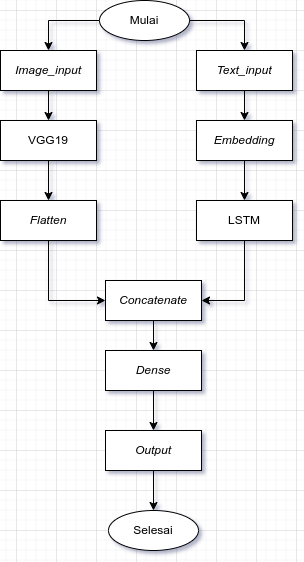
\includegraphics[width = 7cm, height= 14cm]{image/bab4/vgg19-lstm-struktur.png}
  \caption{Struktur arsitektur VGG19-LSTM}
  \label{fig:struktur-arstektur-vgg19-lstm}
\end{figure}

\par Berdasarkan Gambar \ref{fig:struktur-arstektur-vgg19-lstm}, model VGG19-LSTM terdiri dari beberapa lapisan, penjelasan dari setiap lapisan tersebut adalah sebagai berikut:

\begin{enumerate}
  \item Lapisan "\textit{image\_input}" adalah lapisan \textit{input} untuk gambar yang menerima gambar dengan ukuran $224 \times 224$ piksel dan 3 saluran warna (RGB). Lapisan ini tidak memiliki parameter yang bisa dilatih karena hanya berfungsi sebagai \textit{input}.

  \item Lapisan "\textit{text\_input}" adalah lapisan \textit{input} untuk teks yang menerima teks dengan panjang maksimal 24 kata (atau token). Seperti halnya "\textit{image\_input}", lapisan ini juga tidak memiliki parameter yang bisa dilatih karena hanya berfungsi sebagai \textit{input}.

  \item Lapisan "vgg19" adalah model VGG19 yang sudah dilatih sebelumnya, digunakan untuk ekstraksi fitur gambar. \textit{Output} dari lapisan ini adalah tensor dengan dimensi yang belum ditentukan (akan ditentukan saat runtime) dan memiliki 512 fitur. Lapisan ini terhubung ke lapisan "\textit{image\_input}" karena menerima \textit{output} dari lapisan tersebut.

  \item Lapisan "\textit{embedding}" adalah lapisan yang mengubah token teks menjadi vektor \textit{embedding}. \textit{Output} dari lapisan ini adalah tensor dengan panjang 24 dan vektor \textit{embedding} dengan 100 dimensi. Lapisan ini terhubung ke lapisan "\textit{text\_input}" karena menerima \textit{output} dari lapisan tersebut.

  \item Lapisan "\textit{flatten}" adalah lapisan yang mengubah tensor multi-dimensi menjadi vektor 1 dimensi. \textit{Output} dari lapisan ini adalah vektor dengan panjang 25.088. Lapisan ini terhubung ke \textit{output} dari lapisan "vgg19" karena menerima \textit{output} dari lapisan tersebut.

  \item Lapisan "lstm" adalah lapisan LSTM yang mengolah urutan \textit{embedding} teks. \textit{Output} dari lapisan ini adalah tensor dengan 128 unit. Lapisan ini terhubung ke \textit{output} dari lapisan "\textit{embedding}" karena menerima \textit{output} dari lapisan tersebut.

  \item Lapisan "\textit{concatenate}" adalah lapisan yang menggabungkan fitur gambar dan teks. \textit{Output} dari lapisan ini adalah tensor gabungan dengan panjang 25.216. Lapisan ini terhubung ke \textit{output} dari lapisan "flatten" dan "lstm" karena menerima \textit{output} dari kedua lapisan tersebut.

  \item Lapisan "\textit{dense}" setelah lapisan "\textit{concatenate}" adalah lapisan "\textit{dense}" dengan 256 unit. \textit{Output} dari lapisan ini adalah tensor dengan 256 unit. Lapisan ini terhubung ke \textit{output} dari lapisan "\textit{concatenate}" karena menerima \textit{output} dari lapisan tersebut.

  \item Lapisan "\textit{output}" adalah lapisan yang digunakan untuk prediksi akhir dengan 4879 kelas pada \textit{dataset} PathVQA dan 517 kelas pada \textit{dataset} VQA-RAD. \textit{Output} dari lapisan ini adalah tensor dengan 4879 unit (kelas) pada \textit{dataset} PathVQA dan 517 unit (kelas) pada \textit{dataset} VQA-RAD.

\end{enumerate}


\par Struktur dari model VGG19-LSTM yang dilatih dengan \textit{dataset} PathVQA dan VQA-RAD hanya berbeda pada lapisan terakhir, yaitu lapisan "dense" yang memiliki jumlah kelas yang berbeda. Pada \textit{dataset} PathVQA, jumlah kelas yang digunakan adalah 4879 kelas, sedangkan pada \textit{dataset} VQA-RAD, jumlah kelas yang digunakan adalah 517 kelas. Hal ini disebabkan oleh perbedaan jumlah kelas jawaban pada kedua \textit{dataset}. Sehingga, model VGG19-LSTM yang dilatih dengan \textit{dataset} PathVQA memiliki parameter yang lebih banyak dibandingkan dengan model VGG19-LSTM yang dilatih dengan \textit{dataset} VQA-RAD. Jumlah parameter pada model VGG19-LSTM yang dilatih dengan \textit{dataset} PathVQA adalah 27.851.187, sedangkan jumlah parameter pada model VGG19-LSTM yang dilatih dengan \textit{dataset} VQA-RAD adalah 26.730.153.

\par Model ini dikompilasi dengan menggunakan fungsi optimasi Adam dan menggunakan fungsi \textit{loss categorical crossentropy} dikarenakan masalah yang dihadapi adalah masalah klasifikasi multikelas. Dengan adanya fungsi optimasi disini navigasi ruang parameter dapat terjadi yaitu dengan adanya fungsi optimasi yang bekerja dengan menghitung gradien dari fungsi \textit{loss} terhadap masing-masing parameter model. Gradien disini dapat memberitahu fungsi optimasi arah untuk mengubah parameter guna mengurangi \textit{loss}. Secara intuitif, gradien akan menunjukkan arah tercepat untuk turun dari bukit dalam ruang parameter menuju ke titik terendah. Sehingga, model dapat belajar dari data latih dan meningkatkan performa model secara iteratif.

\par Secara keseluruhan, model VGG19-LSTM yang dilatih dengan \textit{dataset} PathVQA dan VQA-RAD memiliki arsitektur yang sama, namun berbeda pada jumlah kelas yang digunakan. Model ini memiliki tiga lapisan utama, yaitu lapisan VGG19, lapisan LSTM, dan lapisan \textit{output} yang digunakan untuk memprediksi jawaban. Model ini memiliki kemampuan untuk memproses gambar dan teks secara bersamaan, dan menghasilkan prediksi jawaban berdasarkan gambar dan pertanyaan yang diberikan.

\subsection{BLIP}

\par Pengembangan model dengan BLIP dilakukan menggunakan pustaka PyTorch versi 2.0.1 dan Transformers versi 4.31.0. Di sini, PyTorch digunakan sebagai \textit{deep learning framework} untuk melatih model, sedangkan Transformers digunakan untuk mengakses \textit{pre-trained} model BLIP. Sebelum melatih model dengan BLIP, penulis melakukan pemrosesan khusus pada data gambar dan data teks menggunakan pustaka Transformers dari Huggingface untuk mengkonversi data tersebut menjadi format yang dapat diproses oleh BLIP. Pustaka Transformers yang digunakan adalah \textit{BlipImageProcessor} dan \textit{BlipProcessor}. Kedua pustaka ini mengkonversi data gambar dan teks menjadi format yang sesuai untuk pemrosesan oleh BLIP.

% \par Dalam arsitektur BLIP, beberapa bagian dari encoder menggunakan GELU (\textit{Gaussian Error Linear Unit}) sebagai fungsi aktivasi. Fungsi aktivasi ini diterapkan antara lapisan-lapisan linear, yang memfasilitasi transformasi input dari satu dimensi ke dimensi lain sebelum memasuki lapisan output. GELU memberikan kontribusi penting dalam meningkatkan performa model berbasis transformer seperti BLIP, karena memungkinkan pemrosesan informasi yang lebih halus dan adaptif. Hal ini membantu model untuk memahami dan mengintegrasikan data dengan lebih efektif, sehingga meningkatkan akurasi dan efisiensi dalam menghasilkan respons yang tepat berdasarkan pertanyaan visual yang diajukan. 

\par Pada model BLIP, data gambar diolah menggunakan \textit{BlipImageProcessor} dari pustaka Transformers. Fungsi \textit{BlipImageProcessor} mengubah ukuran gambar menjadi $128 \times 128$ piksel, dan mengubah gambar yang telah diolah menjadi format tensor yang dapat diproses oleh model BLIP. Sedangkan, untuk data teks diolah menggunakan \textit{BlipProcessor}. Dalam hal ini, \textit{BlipProcessor} melakukan tugas-tugas khusus seperti \textit{padding}, \textit{truncation}, dan \textit{encoding}. \textit{Padding} bertugas menambahkan token khusus pada data teks untuk memastikan bahwa semua data teks memiliki panjang yang sama. \textit{Truncation} bertugas memotong data teks yang melebihi panjang maksimum yang telah ditentukan, yaitu 32 token. \textit{Encoding} mengkonversi data teks menjadi format numerik yang dapat diproses oleh model BLIP.

\par Setelah data gambar dan teks diolah, penulis kemudian mengunduh model yang telah dilatih sebelumnya dari BLIP, yang digunakan untuk tugas \textit{Visual Question Answering} (VQA) menggunakan pustaka Transformers. Model ini dilatih pada \textit{dataset} Visual Genome dan VQA v2.0, dan kemudian dilakukan \textit{fine-tuning} menggunakan \textit{dataset} PathVQA dan VQA-RAD. Dalam proses \textit{fine-tuning} ini, model BLIP dilatih menggunakan fungsi optimasi Adam dan fungsi \textit{loss} \textit{categorical crossentropy}, karena masalah yang dihadapi adalah klasifikasi multikelas. Fungsi optimasi Adam di sini memainkan peran penting dalam meminimalkan nilai \textit{loss} yang dihasilkan oleh fungsi \textit{loss} \textit{categorical crossentropy}. Fungsi \textit{loss} mengukur kesalahan prediksi model terhadap kelas yang sebenarnya, dan nilai \textit{loss} yang lebih rendah menunjukkan kesesuaian yang lebih baik antara prediksi model dan kenyataan. Fungsi optimasi, dalam hal ini Adam, secara efektif mengatur proses pembaharuan bobot model berdasarkan gradien dari fungsi \textit{loss}. Proses ini penting untuk mengarahkan model agar mencapai efisiensi maksimal dalam memprediksi kelas yang benar, secara bertahap menurunkan kesalahan prediksi sepanjang iterasi pelatihan. Oleh karena itu, pemilihan fungsi optimasi yang tepat sangat krusial untuk memastikan keberhasilan \textit{fine-tuning} model dalam mencapai hasil yang akurat dan relevan. 

\par Struktur model BLIP pada tugas \textit{Visual Question Answering (VQA)} terdiri dari tiga lapisan utama, yaitu \textit{vision\_model}, \textit{text\_encoder}, dan \textit{text\_decoder}. Ketiga lapisan ini berfungsi untuk memproses \textit{input} gambar dan teks, serta menghasilkan prediksi jawaban akhir berdasarkan gambar dan pertanyaan yang diberikan. Struktur dari ketiga lapisan ini dapat dilihat pada Lampiran 1, Lampiran 2, dan Lampiran 3.


\par Lapisan \textit{vision\_model} bertugas untuk memproses \textit{input} gambar dan terdiri dari dua bagian utama: \textit{embeddings} dan \textit{encoder}. Di bagian \textit{embeddings} menggunakan \textit{backbone Vision Transformer} (ViT) untuk mengubah gambar menjadi \textit{patch embedding}. Bagian \textit{encoder} terdiri dari beberapa lapisan \textit{encoder} yang menangkap hubungan antar \textit{patch} gambar menggunakan mekanisme \textit{self-attention}. Setiap \textit{layer encoder} dilengkapi dengan normalisasi dan \textit{Multi-Layer Perceptron} (MLP) dengan aktivasi \textit{Gaussian Error Linear Unit} (GELU) untuk transformasi lebih lanjut. Berikut adalah penjelasan dari setiap lapisan dalam \textit{vision\_model}:

\begin{enumerate}

    \item \textit{Embeddings}: Ini merupakan komponen dari \textit{BlipVisionModel} yang menggunakan \textit{BlipVisionEmbeddings} untuk menerapkan konvolusi 2D (Conv2d) dengan menggunakan \textit{backbone} ViT untuk mengubah gambar menjadi representasi vektor dari potongan-potongan gambar (\textit{patches}).

    \item \textit{BlipVisionEmbeddings}: Ini merupakan komponen yang mencakup \textit{patch embeddings} menggunakan Conv2d. Dimensi \textit{input} adalah 3 saluran warna RGB, dimensi \textit{output} adalah 768, ukuran kernel $16 \times 16$, dan stride $16 \times 16$.

    \item \textit{Encoder}: Bagian yang mencakup \textit{BlipEncoder} yang terdiri dari beberapa lapisan \textit{encoder} yang masing-masing menggunakan mekanisme \textit{self-attention} untuk menangkap hubungan antar \textit{patch} gambar.

    \item \textit{BlipEncoder}: Ini merupakan komponen utama \textit{encoder} yang terdiri dari beberapa \textit{BlipEncoderLayer}, dengan jumlah total 12 lapisan.

    \item \textit{BlipEncoderLayer}: Bagian dari \textit{BlipEncoder} yang dimana setiap lapisan yang terdiri dari bagian terdapat beberapa subkomponen yaitu \textit{self-attention}, MLP, dua \textit{LayerNorm}. Di bagian ini, \textit{input} dari gambar diolah menggunakan mekanisme \textit{self-attention} dan MLP untuk transformasi lebih lanjut.

    \item \textit{BlipAttention}: Bagian ini menangkap hubungan antar \textit{patch} gambar menggunakan mekanisme \textit{self-attention}. Komponen ini menggunakan \textit{query}, \textit{key}, dan \textit{value} dengan dimensi $768 \times 2304$ dan proyeksi dengan dimensi $768 \times 768$. Nilai \textit{dropout} adalah 0,0.

    \item \textit{BlipMLP}: Menggunakan lapisan linear untuk transformasi lebih lanjut dari hasil \textit{attention} dan fungsi aktivasi GELU untuk menambah non-linearitas. Lapisan pertama (fc1) memiliki dimensi $768 \times 3072$ dan lapisan kedua (fc2) memiliki dimensi $3072 \times 768$.

    \item \textit{LayerNorm}: Digunakan untuk normalisasi pada beberapa bagian model, termasuk \textit{layer\_norm1}, \textit{layer\_norm2}, dan \textit{post\_layernorm}. Parameter \textit{LayerNorm} memiliki nilai epsilon $1 \times 10^{-5}$.

    \item \textit{PostLayerNorm}: Merupakan lapisan normalisasi akhir setelah seluruh lapisan \textit{encoder} selesai memproses \textit{input}. Tujuannya adalah untuk menstabilkan dan menormalisasi keluaran akhir dari \textit{encoder} sebelum digunakan oleh bagian lain dari model.


  
\end{enumerate}

\par Lapisan \textit{text\_encoder} bertugas untuk memproses \textit{input} teks dan terdiri dari dua bagian utama: \textit{embeddings} dan \textit{encoder}. Bagian \textit{embeddings} menyediakan representasi kata dan posisi dalam teks, sementara bagian \textit{encoder} terdiri dari beberapa lapisan yang menangkap hubungan antar kata menggunakan mekanisme \textit{attention}. Selain \textit{self-attention}, terdapat \textit{cross-attention} yang menangkap hubungan antara teks dan fitur gambar jika ada. Setiap \textit{layer encoder} juga dilengkapi dengan normalisasi dan MLP untuk transformasi lebih lanjut. Berikut adalah penjelasan dari setiap lapisan dalam \textit{text\_encoder}:

\begin{enumerate}

  \item \textit{Embeddings}: Pada bagian ini terdiri dari \textit{word embeddings} yang merupakan representasi vektor dari kata-kata dalam teks dan \textit{position embeddings} yang memberikan informasi posisi dari setiap kata dalam teks. Jumlah fitur yang digunakan adalah 768 dengan \textit{padding} indeks 0.

  \item \textit{BlipTextEmbeddings}: Ini merupakan komponen yang mencakup \textit{word embeddings} dan \textit{position embeddings}, serta menggunakan \textit{LayerNorm} untuk normalisasi dan \textit{dropout} untuk mengurangi \textit{overfitting}. Dimensi \textit{word embeddings} adalah $30524 \times 768$ dimensi, sedangkan dimensi \textit{position embeddings} adalah $512 \times 768$ dimensi. Parameter \textit{LayerNorm} memiliki nilai epsilon $1 \times 10^{-12}$, dengan nilai \textit{dropout} 0,0.

  \item \textit{Encoder}: Pada bagian ini terdiri dari beberapa lapisan yang masing-masing menggunakan mekanisme \textit{attention} untuk menangkap hubungan antar kata. Hal ini bertujuan untuk memahami dan mengintegrasikan informasi pada pertanyaan yang diajukan.

  \item \textit{BlipTextEncoder}: Ini merupakan komponen \textit{encoder} yang terdiri dari beberapa lapisan \textit{BlipTextLayer}. 

  \item \textit{BlipTextLayer}: Setiap lapisan terdiri dari beberapa subkomponen yaitu \textit{attention}, \textit{crossattention}, \textit{intermediate}, dan \textit{output}, dengan jumlah total 12 lapisan \textit{BlipTextLayer}.

  \item \textit{BlipTextAttention}: Hal ini berguna untuk menangkap hubungan antar kata dalam teks menggunakan \textit{self-attention} dan hubungan antara teks dan fitur gambar menggunakan \textit{cross-attention}. Dimensi \textit{query}, \textit{key}, dan \textit{value} masing-masing adalah $768 \times 768$ dengan nilai \textit{dropout} 0,0.

  \item \textit{BlipTextSelfAttention}: Bagian dari \textit{BlipTextAttention} yang menggunakan \textit{query}, \textit{key}, dan \textit{value} untuk menghitung perhatian antar kata dalam teks, dengan dimensi \textit{query}, \textit{key}, dan \textit{value} masing-masing $768 \times 768$.

  \item \textit{BlipTextSelfOutput}: Bagian ini menghasilkan \textit{output} dari mekanisme \textit{attention} dan menggunakan \textit{LayerNorm} serta \textit{dropout} untuk normalisasi dan mengurangi \textit{overfitting}. Dimensi dense layer adalah $768 \times 768$ dengan parameter \textit{LayerNorm} epsilon $1 \times 10^{-12}$ dan nilai \textit{dropout} 0,0.

  \item \textit{BlipTextIntermediate}: Bagian ini menggunakan lapisan linear untuk transformasi lebih lanjut dari hasil \textit{attention} dan fungsi aktivasi GELU untuk menambah non-linearitas. Dimensi dense layer adalah $768 \times 3072$ dengan fungsi aktivasi GELU.

  \item \textit{BlipTextOutput}: Di sini dihasilkan \textit{output} akhir dari lapisan \textit{encoder} dengan lapisan linear dan \textit{LayerNorm} untuk normalisasi. Dimensi dense layer adalah $3072 \times 768$ dengan parameter \textit{LayerNorm} epsilon $1 \times 10^{-12}$ serta nilai \textit{dropout} 0,0.


\end{enumerate}



\par Lapisan \textit{text\_decoder} bertugas untuk mendekode dan menghasilkan teks dari fitur yang telah diproses, menggunakan struktur yang mirip dengan model \textit{Bidirectional Encoder Representation From Transformers} (BERT). Bagian \textit{decoder} terdiri dari \textit{embeddings} untuk kata dan posisi, serta beberapa lapisan \textit{encoder} yang menggunakan mekanisme \textit{self-attention} dan \textit{cross-attention}. Setiap lapisan dilengkapi dengan MLP dan normalisasi untuk transformasi lebih lanjut. Bagian \textit{cls} dari \textit{decoder} bertugas untuk menghasilkan prediksi jawaban akhir berdasarkan fitur yang telah diproses. Berikut adalah penjelasan dari setiap lapisan dalam \textit{text\_decoder}:

\begin{enumerate}

  \item \textit{Embeddings}: Menggunakan \textit{word embeddings} dan \textit{position embeddings} untuk menyediakan representasi vektor dari kata dan posisi dalam teks. Pada bagian ini, dimensi pada \textit{word embeddings} adalah $30524 \times 768$, sedangkan dimensi \textit{position embeddings} adalah $512 \times 768$. Lapisan ini juga menggunakan \textit{LayerNorm} dengan nilai epsilon $1 \times 10^{-12}$ dan \textit{dropout} dengan nilai 0,0.

  \item \textit{BlipTextEmbeddings}: Bagian ini, merupakan komponen utama yang mencakup \textit{word embeddings} dan \textit{position embeddings}, serta menggunakan \textit{LayerNorm} dan \textit{dropout} untuk normalisasi dan mengurangi \textit{overfitting}. Pada bagian ini, dimensi \textit{word embeddings} adalah $30524 \times 768$, dimensi \textit{position embeddings} adalah $512 \times 768$, nilai epsilon $1 \times 10^{-12}$, dan nilai \textit{dropout} 0,0.

  \item \textit{Encoder}: Terdiri dari beberapa lapisan \textit{encoder} yang menggunakan mekanisme \textit{self-attention} dan \textit{cross-attention} untuk menangkap hubungan antar kata dan antara kata dengan fitur lain. Terdapat total 12 lapisan \textit{BlipTextLayer}.

  \item \textit{BlipTextEncoder}: Ini merupakan komponen utama \textit{encoder} yang terdiri dari beberapa \textit{BlipTextLayer}, dengan jumlah total 12 lapisan.

  \item \textit{BlipTextLayer}: Setiap lapisan terdiri dari beberapa subkomponen yaitu \textit{attention}, \textit{crossattention}, \textit{intermediate}, dan \textit{output}. Lapisan \textit{attention} dan \textit{crossattention} masing-masing menggunakan \textit{self-attention} dengan \textit{query}, \textit{key}, dan \textit{value}, serta proyeksi dengan dimensi $768 \times 768$ dan nilai \textit{dropout} 0,0. Lapisan \textit{intermediate} menggunakan lapisan linear dengan dimensi $768 \times 3072$ dan fungsi aktivasi GELU, sementara lapisan \textit{output} menggunakan lapisan linear dengan dimensi $3072 \times 768$ dan \textit{LayerNorm} dengan nilai epsilon $1 \times 10^{-12}$.

  \item \textit{BlipTextAttention}: Hal ini berguna untuk menangkap hubungan antar kata dalam teks menggunakan mekanisme \textit{self-attention}. Komponen ini menggunakan \textit{query}, \textit{key}, dan \textit{value} dengan dimensi $768 \times 768$ dan proyeksi dengan dimensi $768 \times 768$. Nilai \textit{dropout} adalah 0,0.

  \item \textit{BlipTextSelfAttention}: Bagian dari \textit{BlipTextAttention} yang menggunakan \textit{query}, \textit{key}, dan \textit{value} untuk menghitung perhatian antar kata dalam teks, dengan dimensi \textit{query}, \textit{key}, dan \textit{value} masing-masing $768 \times 768$.

  \item \textit{BlipTextSelfOutput}: Bagian ini, menghasilkan \textit{output} dari mekanisme \textit{attention} dan menggunakan \textit{LayerNorm} serta \textit{dropout} untuk normalisasi dan mengurangi \textit{overfitting}. Dimensi dense layer adalah $768 \times 768$ dengan parameter \textit{LayerNorm} epsilon $1 \times 10^{-12}$ serta nilai \textit{dropout} 0,0.

  \item \textit{BlipTextIntermediate}: Menggunakan lapisan linear untuk transformasi lebih lanjut dari hasil \textit{attention} dan fungsi aktivasi GELU untuk menambah non-linearitas. Dimensi dense layer adalah $768 \times 3072$ dengan fungsi aktivasi GELU.

  \item \textit{BlipTextOutput}: Menghasilkan \textit{output} akhir dari lapisan \textit{encoder} dengan lapisan linear dan \textit{LayerNorm} untuk normalisasi. Dimensi dense layer adalah $3072 \times 768$ dengan parameter \textit{LayerNorm} epsilon $1 \times 10^{-12}$ serta nilai \textit{dropout} 0,0.

  \item \textit{BlipTextOnlyMLMHead}: Bertugas untuk menghasilkan prediksi jawaban akhir berdasarkan fitur yang telah diproses. Bagian dari komponen ini mencakup \textit{BlipTextLMPredictionHead} yang terdiri dari transformasi dan \textit{decoder}. Transform menggunakan lapisan linear dengan dimensi $768 \times 768$, fungsi aktivasi GELU, dan \textit{LayerNorm} dengan nilai epsilon $1 \times 10^{-12}$. Bagian \textit{decoder} menggunakan lapisan linear dengan dimensi $768 \times 30524$.

  \item \textit{BlipTextLMPredictionHead}: Ini merupakan komponen dari \textit{cls} yang mencakup transformasi dan \textit{decoder}. Disini, dilakukan transformasi dengan menggunakan lapisan linear dengan dimensi $768 \times 768$, fungsi aktivasi GELU, dan \textit{LayerNorm} dengan nilai epsilon $1 \times 10^{-12}$. Disini, \textit{decoder} menggunakan lapisan linear dengan dimensi $768 \times 30524$.

  \item \textit{BlipTextPredictionHeadTransform}: Bagian dari \textit{BlipTextLMPredictionHead} yang menggunakan lapisan linear untuk transformasi fitur dengan dimensi $768 \times 768$, fungsi aktivasi GELU, dan \textit{LayerNorm} dengan nilai epsilon $1 \times 10^{-12}$.

\end{enumerate}

Secara keseluruhan, model BLIP pada tugas VQA yang terdiri dari tiga lapisan utama, yaitu \textit{vision\_model}, \textit{text\_encoder}, dan \textit{text\_decoder}, berguna untuk memproses kedua \textit{input} yaitu gambar dan pertanyaan, serta menghasilkan prediksi jawaban akhir berdasarkan kedua \textit{input} tersebut. Dengan adanya tiga lapisan ini, model BLIP dapat memahami dan merespon pertanyaan visual dengan lebih efektif dan efisien, sehingga meningkatkan akurasi dan relevansi jawaban yang dihasilkan, sehingga dapat membantu dalam mendukung pertanyaan dengan konteks visual yang ada.

\section{Augmentasi Data}

\par Pada penelitian ini, dilakukan augmentasi data untuk kalimat pertanyaan pada \textit{dataset} PathVQA dan VQA-RAD. Augmentasi ini menggunakan teknik augmentasi teks dari pustaka nlpaug versi 1.1.11. Teknik ini memanfaatkan fungsi dari nlpaug untuk menghasilkan variasi parafrase dari setiap pertanyaan dalam \textit{dataset}. Pada penelitian ini, setiap pertanyaan diubah menjadi tujuh variasi yang berbeda. Setiap versi parafrase dari pertanyaan tersebut kemudian dibuat sebagai entri baru dalam \textit{dataset}, di mana setiap entri baru masih mengacu pada gambar dan jawaban yang sama dengan pertanyaan asli. Metode augmentasi ini meningkatkan variasi linguistik dalam \textit{dataset}, yang sangat bermanfaat untuk melatih model NLP agar dapat memahami dan merespon berbagai formulasi pertanyaan secara lebih efektif. Augmentasi dilakukan dengan menggunakan sinonim dari leksikal WordNet untuk menghasilkan sinonim untuk kata-kata dalam kalimat yang ada, sehingga menghasilkan variasi parafrase dari kalimat asli. Pada saat proses augmentasi ada bermunculan data yang duplikat, oleh karena itu penulis melakukan penghapusan data duplikat tersebut. Dengan menerapkan teknik augmentasi ini, awalnya \textit{dataset} PathVQA memiliki 32.632 data, setelah dilakukan augmentasi data menjadi 179.167 data. Sedangkan \textit{dataset} VQA-RAD yang awalnya memiliki 2.248 data, setelah dilakukan augmentasi data menjadi 14.347 data. Pada hal ini tujuan dilakukan augmentasi data karena pertanyaan terkait masalah medis sangatlah beragam dan kompleks, sehingga diperlukan variasi pertanyaan yang lebih banyak dan mengatasi kurangnya variasi pertanyaan pada \textit{dataset} yang ada. Pada Tabel \ref{tab:augmentasi-data} menunjukkan contoh pertanyaan yang telah diaugmentasi dengan memanfaatkan teknik augmentasi teks dari pustaka nlpaug dengan menggunakan sinonim dari leksikal WordNet.

% Please add the following required packages to your document preamble:
% \usepackage{multirow}
% \usepackage{graphicx}
\begin{table}[H]
  \centering
  \caption{Contoh pertanyaan yang telah diaugmentasi}
  \label{tab:augmentasi-data}
  \resizebox{\textwidth}{!}{%
  \begin{tabular}{|l|l|}
  \hline
  \textbf{Pertanyaan original} & \textbf{Pertanyaan augmentasi}                                                                                                        \\ \hline
  \multirow{7}{*}{\textit{\begin{tabular}[c]{@{}l@{}}What is the primary use of MRI \\ in medical diagnosis?\end{tabular}}} &
    \textit{\begin{tabular}[c]{@{}l@{}}What is the elemental use of magnetic resonance\\ imaging in aesculapian diagnosis?\end{tabular}} \\ \cline{2-2} 
                               & \textit{\begin{tabular}[c]{@{}l@{}}What be the primary usance of magnetic resonance\\ imaging in medical diagnosis?\end{tabular}}     \\ \cline{2-2} 
                               & \textit{\begin{tabular}[c]{@{}l@{}}What embody the main use of magnetic resonance\\ imaging in aesculapian diagnosis?\end{tabular}}   \\ \cline{2-2} 
                               & \textit{\begin{tabular}[c]{@{}l@{}}What is the primary habit of magnetic resonance \\ imaging in medical diagnosis?\end{tabular}}     \\ \cline{2-2} 
                               & \textit{What be the primary use of MRI in medical diagnosis?}                                                                         \\ \cline{2-2} 
                               & \textit{\begin{tabular}[c]{@{}l@{}}What is the primary usance of magnetic resonance\\ imaging in aesculapian diagnosis?\end{tabular}} \\ \cline{2-2} 
                               & \textit{\begin{tabular}[c]{@{}l@{}}What be the primary use of magnetic resonance\\ imaging in medical diagnosis?\end{tabular}}        \\ \hline
  \end{tabular}%
  }
  \end{table}


\section{Analisis Hasil}

\par Dalam rangka melakukan eksperimen, penulis telah melakukan konfigurasi dari berbagai \textit{hyperparameter} untuk melatih model VGG19-LSTM dan BLIP, dengan tujuan meningkatkan efektivitas dan efisiensi pelatihan. Dalam hal ini, \textit{hyperparameter} yang diatur mencakup jumlah \textit{epochs}, \textit{learning rate}, dan \textit{batch size}. Peran ketiga \textit{hyperparameter} ini memiliki peran penting dalam menentukan keberhasilan pelatihan model, karena mempengaruhi proses optimisasi model untuk mencapai hasil yang optimal. \textit{Hyperparameter} ini memungkinkan penyesuaian yang lebih spesifik terhadap karakteristik data dan kebutuhan eksperimental, sehingga memungkinkan model untuk belajar dengan lebih baik dan menghasilkan respons yang lebih akurat terhadap pertanyaan visual yang diajukan. Tabel \ref{tab:konfigurasi-hyperparameter-model} menunjukkan konfigurasi \textit{hyperparameter} yang digunakan dalam eksperimen ini untuk melatih model VGG19-LSTM dan BLIP dengan \textit{dataset} PathVQA dan VQA-RAD, sebelum dilakukan augmentasi data. Hal ini dilakukan untuk melihat pengaruh konfigurasi \textit{hyperparameter} terhadap performa model pada data asli sebelum dilakukan augmentasi.
  
% Please add the following required packages to your document preamble:
% \usepackage{multirow}
\begin{table}[H]
  \centering
  \caption{Konfigurasi \textit{hyperparameter} pada awal eksperimen}  
  \label{tab:konfigurasi-hyperparameter-model}
  \begin{tabular}{|c|ccc|}
  \hline
  \multirow{2}{*}{\textbf{No}} & \multicolumn{3}{c|}{\textbf{Konfigurasi \textit{hyperparameter}}} \\ \cline{2-4} 
   & \multicolumn{1}{c|}{\textbf{\textit{Epochs}}} & \multicolumn{1}{c|}{\textbf{\textit{Learning rate}}} & \textbf{\textit{Batch size}} \\ \hline
  \multirow{6}{*}{1} & \multicolumn{1}{c|}{\multirow{6}{*}{15}} & \multicolumn{1}{c|}{\multirow{3}{*}{$1 \times 10^{-5}$}} & 8 \\ \cline{4-4} 
   & \multicolumn{1}{c|}{} & \multicolumn{1}{c|}{} & 16 \\ \cline{4-4} 
   & \multicolumn{1}{c|}{} & \multicolumn{1}{c|}{} & 32 \\ \cline{3-4} 
   & \multicolumn{1}{c|}{} & \multicolumn{1}{c|}{\multirow{3}{*}{$5 \times 10^{-5}$}} & 8 \\ \cline{4-4} 
   & \multicolumn{1}{c|}{} & \multicolumn{1}{c|}{} & 16 \\ \cline{4-4} 
   & \multicolumn{1}{c|}{} & \multicolumn{1}{c|}{} & 32 \\ \hline
  \multirow{6}{*}{2} & \multicolumn{1}{c|}{\multirow{6}{*}{30}} & \multicolumn{1}{c|}{\multirow{3}{*}{$1 \times 10^{-5}$}} & 8 \\ \cline{4-4} 
   & \multicolumn{1}{c|}{} & \multicolumn{1}{c|}{} & 16 \\ \cline{4-4} 
   & \multicolumn{1}{c|}{} & \multicolumn{1}{c|}{} & 32 \\ \cline{3-4} 
   & \multicolumn{1}{c|}{} & \multicolumn{1}{c|}{\multirow{3}{*}{$5 \times 10^{-5}$}} & 8 \\ \cline{4-4} 
   & \multicolumn{1}{c|}{} & \multicolumn{1}{c|}{} & 16 \\ \cline{4-4} 
   & \multicolumn{1}{c|}{} & \multicolumn{1}{c|}{} & 32 \\ \hline
  \multirow{6}{*}{3} & \multicolumn{1}{c|}{\multirow{6}{*}{45}} & \multicolumn{1}{c|}{\multirow{3}{*}{$1 \times 10^{-5}$}} & 8 \\ \cline{4-4} 
   & \multicolumn{1}{c|}{} & \multicolumn{1}{c|}{} & 16 \\ \cline{4-4} 
   & \multicolumn{1}{c|}{} & \multicolumn{1}{c|}{} & 32 \\ \cline{3-4} 
   & \multicolumn{1}{c|}{} & \multicolumn{1}{c|}{\multirow{3}{*}{$5 \times 10^{-5}$}} & 8 \\ \cline{4-4} 
   & \multicolumn{1}{c|}{} & \multicolumn{1}{c|}{} & 16 \\ \cline{4-4} 
   & \multicolumn{1}{c|}{} & \multicolumn{1}{c|}{} & 32 \\ \hline
  \end{tabular}
  \end{table}


\par Konfigurasi \textit{hyperparameter} yang digunakan dalam eksperimen ini merupakan pilihan berdasarkan preferensi peneliti untuk mendapatkan kombinasi awal yang rasional. Eksperimen dengan jumlah \textit{epochs} 15, 30, dan 45, \textit{batch size} 8, 16, dan 32, serta \textit{learning rate} sebesar $1 \times 10^{-5}$, dan $5 \times 10^{-5}$. Dengan menggunakan kombinasi \textit{hyperparameter} ini, penulis akan mencari kombinasi yang paling optimal dengan menggunakan metode \textit{grid search} untuk mencari kombinasi \textit{hyperparameter} yang paling optimal.


\par Dari hasil eksperimen yang dilakukan dengan VGG19-LSTM dengan \textit{dataset} PathVQA dan VQA-RAD didapatlah hasil untuk pengujian pada pertanyaan yang bersifat \textit{close-ended} dapat dilihat pada Lampiran 4, sedangkan untuk pengujian pada pertanyaan yang bersifat \textit{open-ended} dapat dilihat pada Lampiran 5, dan untuk pengujian pada keseluruhan pertanyaan dapat dilihat pada Lampiran 6. Dari hasil eksperimen tersebut, dapat dilihat bahwa beberapa hasil akurasi dari model VGG19-LSTM dengan \textit{dataset} PathVQA dan VQA-RAD dapat dilihat pada Tabel \ref{tab:sepuluh-hasil-terbaik-vgg19-lstm}. Pada Tabel \ref{tab:sepuluh-hasil-terbaik-vgg19-lstm-bleu} disajikan informasi mengenai hasil BLEU pada pertanyaan \textit{open-ended} dengan VGG19-LSTM. Tabel \ref{tab:sepuluh-hasil-terbaik-vgg19-lstm-bleu} menunjukkan beberapa hasil terbaik dari model VGG19-LSTM dengan \textit{dataset} PathVQA dan VQA-RAD berdasarkan nilai BLEU-1, BLEU-2, dan BLEU-3 untuk melihat kualitas jawaban yang bersifat \textit{open-ended} yang dihasilkan oleh model.

% Please add the following required packages to your document preamble:
% \usepackage{multirow}
\begin{table}[H]
  \centering
  \caption{Hasil akurasi pelatihan dengan VGG19-LSTM}
  \label{tab:sepuluh-hasil-terbaik-vgg19-lstm}
  \begin{tabular}{|c|l|l|l|l|l|l|}
  \hline
  \multicolumn{1}{|l|}{\textit{\textbf{Dataset}}} & \textit{\textbf{Epochs}} & \textit{\textbf{\begin{tabular}[c]{@{}l@{}}Batch \\ size\end{tabular}}} & \textit{\textbf{\begin{tabular}[c]{@{}l@{}}Learning \\ rate\end{tabular}}} & \textbf{Akurasi} & \textbf{\begin{tabular}[c]{@{}l@{}}Akurasi \\ \textit{close}\\ \textit{ended}\end{tabular}} & \textbf{\begin{tabular}[c]{@{}l@{}}Akurasi\\ \textit{open}\\ \textit{ended}\end{tabular}} \\ \hline
  \multirow{5}{*}{PathVQA} & 15 & 8 & $1 \times 10^{-5}$ & 26,96\% & 43,02\% & 10,16\% \\ \cline{2-7} 
   & 15 & 8 & $5 \times 10^{-5}$ & 37,07\% & 53,44\% & 19,90\% \\ \cline{2-7} 
   & 45 & 16 & $5 \times 10^{-5}$ & 35,39\% & 51,23\% & 19,77\% \\ \cline{2-7} 
   & 45 & 8 & $5 \times 10^{-5}$ & 35,20\% & 48,66\% & 22,15\% \\ \cline{2-7} 
   & 15 & 16 & $5 \times 10^{-5}$ & 34,68\% & 51,44\% & 18,53\% \\ \hline
  \multirow{5}{*}{VQA-RAD} & 30 & 8 & $5 \times 10^{-5}$ & 46,67\% & 69,05\% & 18,18\% \\ \cline{2-7} 
   & 45 & 16 & $5 \times 10^{-5}$ & 45,78\% & 66,93\% & 18,37\% \\ \cline{2-7} 
   & 45 & 8 & $5 \times 10^{-5}$ & 41,78\% & 71,05\% & 11,71\% \\ \cline{2-7} 
   & 45 & 32 & $5 \times 10^{-5}$ & 41,33\% & 68,75\% & 14,16\% \\ \cline{2-7} 
   & 45 & 8 & $1 \times 10^{-5}$ & 39,11\% & 62,81\% & 11,54\% \\ \hline
  \end{tabular}
  \end{table}
  
\par \textit{Baseline} model yang digunakan dalam eksperimen dengan menggunakan VGG19-LSTM adalah model yang dilatih pada \textit{dataset} PathVQA dan VQA-RAD dengan \textit{hyperparameter} \textit{epochs} 15, \textit{batch size} 8, dan \textit{learning rate} $1 \times 10^{-5}$. Model ini digunakan sebagai pembanding untuk melihat apakah model yang dilatih dengan konfigurasi \textit{hyperparameter} yang berbeda dapat menghasilkan performa yang lebih baik. Dari hasil eksperimen yang dilakukan, dapat dilihat bahwa model VGG19-LSTM yang memiliki nilai akurasi terbaik pada \textit{dataset} PathVQA adalah ketika \textit{epochs} 45, \textit{batch size} 8, dan \textit{learning rate} $5 \times 10^{-5}$ dengan akurasi 37,07\%, akurasi \textit{close-ended} 53,44\%, dan akurasi \textit{open-ended} 19,90\%. Pada \textit{dataset} VQA-RAD adalah ketika \textit{epochs} 30, \textit{batch size} 8, dan \textit{learning rate} $5 \times 10^{-5}$ dengan akurasi 46,67\%, akurasi \textit{close-ended} 69,05\%, dan akurasi \textit{open-ended} 18,18\%.

% Please add the following required packages to your document preamble:
% \usepackage{multirow}
\begin{table}[H]
  \centering
  \caption{Hasil BLEU pada pertanyaan open-ended dengan VGG19-LSTM}
  \label{tab:sepuluh-hasil-terbaik-vgg19-lstm-bleu}
  \begin{tabular}{|c|l|l|l|l|l|l|}
  \hline
  \multicolumn{1}{|l|}{\textit{\textbf{Dataset}}} & \textit{\textbf{Epochs}} & \textit{\textbf{\begin{tabular}[c]{@{}l@{}}Batch \\ size\end{tabular}}} & \textit{\textbf{\begin{tabular}[c]{@{}l@{}}Learning \\ rate\end{tabular}}} & \textbf{BLEU-1} & \textbf{BLEU-2} & \textbf{BLEU-3} \\ \hline
  \multirow{5}{*}{PathVQA} & 15 & 8 & $1 \times 10^{-5}$ & 10,89 & 3,86 & 2,57 \\ \cline{2-7} 
   & 15 & 8 & $5 \times 10^{-5}$ & 21,41 & 8,01 & 5,38 \\ \cline{2-7} 
   & 45 & 16 & $5 \times 10^{-5}$ & 22,32 & 9,63 & 6,72 \\ \cline{2-7} 
   & 45 & 8 & $5 \times 10^{-5}$ & 24,28 & 10,02 & 6,81 \\ \cline{2-7} 
   & 15 & 16 & $5 \times 10^{-5}$ & 19,95 & 7,96 & 5,23 \\ \hline
  \multirow{5}{*}{VQA-RAD} & 30 & 8 & $5 \times 10^{-5}$ & 20,17 & 14,34 & 11,32 \\ \cline{2-7} 
   & 45 & 16 & $5 \times 10^{-5}$ & 20,69 & 16,69 & 11,29 \\ \cline{2-7} 
   & 45 & 8 & $5 \times 10^{-5}$ & 13,08 & 7,45 & 4,74 \\ \cline{2-7} 
   & 45 & 32 & $5 \times 10^{-5}$ & 15,16 & 11,64 & 7,85 \\ \cline{2-7} 
   & 45 & 8 & $1 \times 10^{-5}$ & 12,26 & 7,23 & 5,51 \\ \hline
  \end{tabular}
\end{table}

\par Pada Tabel \ref{tab:sepuluh-hasil-terbaik-vgg19-lstm-bleu} dapat dilihat bahwa model VGG19-LSTM yang memiliki nilai BLEU terbaik pada \textit{dataset} PathVQA adalah ketika \textit{epochs} 45, \textit{batch size} 8, dan \textit{learning rate} $5 \times 10^{-5}$ dengan BLEU-1 24,28, BLEU-2 10,02, BLEU-3 6,81. Dari hasil ini, dapat diinterpretasikan bahwa model VGG19-LSTM ketika mengevaluasi jawaban untuk kata tunggal, model mampu menunjukkan bahwa intisari terjemahan cukup jelas meskipun terdapat kesalahan tata bahasa yang signifikan, dikarenakan nilai BLEU-1 yang didapat adalah 24,28. Sementara itu, nilai BLEU-2 yang tercatat sebesar 10,02 menandakan bahwa model sulit untuk memahami pasangan dua kata yang berurutan. Lalu, nilai BLEU-3 yang tercatat sebesar 6,81 menandakan bahwa model hampir tidak mampu memahami frasa tiga kata yang berurutan. 

\par Berdasarkan Tabel \ref{tab:sepuluh-hasil-terbaik-vgg19-lstm-bleu} dapat dilihat bahwa model VGG19-LSTM yang memiliki nilai BLEU terbaik pada \textit{dataset} VQA-RAD adalah ketika \textit{epochs} ketika \textit{epochs} 45, \textit{batch size} 16, dan \textit{learning rate} $5 \times 10^{-5}$ dengan BLEU-1 20,69, BLEU-2 16,69, dan BLEU-3 11,29. Dari hasil ini, dapat diinterpretasikan bahwa model VGG19-LSTM ketika mengevaluasi jawaban untuk kata tunggal, model mampu menunjukkan bahwa intisari terjemahan cukup jelas meskipun terdapat kesalahan tata bahasa yang signifikan, dikarenakan nilai BLEU-1 yang didapat adalah 20,69. Sementara itu, nilai BLEU-2, dan BLEU-3 yang tercatat sebesar 16,69 dan 11,29 menandakan bahwa model sulit untuk memahami pasangan dua kata yang berurutan dan frasa tiga kata yang berurutan.  

\par Dari hasil eksperimen yang dilakukan, dapat dilihat bahwa setelah dilakukan \textit{hyperparameter tuning}, model VGG19-LSTM yang dilatih dengan \textit{dataset} PathVQA dan VQA-RAD menghasilkan performa yang lebih baik dibandingkan dengan \textit{baseline} model. Hal ini menunjukkan bahwa konfigurasi \textit{hyperparameter} yang tepat dapat meningkatkan performa model dalam memprediksi jawaban dari pertanyaan yang diberikan.

\par Eksperimen yang dilakukan dengan BLIP dengan \textit{dataset} PathVQA dan VQA-RAD didapatlah hasil untuk pengujian pada pertanyaan yang bersifat \textit{close-ended} dapat dilihat pada Lampiran 7, sedangkan untuk pengujian pada pertanyaan yang bersifat \textit{open-ended} dapat dilihat pada Lampiran 8, dan untuk pengujian pada keseluruhan pertanyaan dapat dilihat pada Lampiran 9. Dari hasil eksperimen tersebut, dapat dilihat bahwa beberapa hasil dari model BLIP dengan \textit{dataset} PathVQA dan VQA-RAD dapat dilihat pada Tabel \ref{tab:sepuluh-hasil-terbaik-blip}. Tabel \ref{tab:sepuluh-hasil-terbaik-blip-bleu} disajikan informasi mengenai hasil BLEU pada pertanyaan \textit{open-ended} dengan BLIP. Tabel \ref{tab:sepuluh-hasil-terbaik-blip-bleu} menunjukkan beberapa hasil terbaik dari model BLIP dengan \textit{dataset} PathVQA dan VQA-RAD berdasarkan nilai BLEU-1, BLEU-2, dan BLEU-3 untuk melihat kualitas jawaban yang bersifat \textit{open-ended} yang dihasilkan oleh model.

% Please add the following required packages to your document preamble:
% \usepackage{multirow}
\begin{table}[H]
  \centering
  \caption{Hasil akurasi pelatihan dengan BLIP}
  \label{tab:sepuluh-hasil-terbaik-blip}
  \begin{tabular}{|c|l|l|l|l|l|l|}
  \hline
  \multicolumn{1}{|l|}{\textit{\textbf{Dataset}}} & \textit{\textbf{Epochs}} & \textit{\textbf{\begin{tabular}[c]{@{}l@{}}Batch \\ size\end{tabular}}} & \textit{\textbf{\begin{tabular}[c]{@{}l@{}}Learning \\ rate\end{tabular}}} & \textbf{Akurasi} & \textbf{\begin{tabular}[c]{@{}l@{}}Akurasi \\ \textit{close}\\ \textit{ended}\end{tabular}} & \textbf{\begin{tabular}[c]{@{}l@{}}Akurasi\\ \textit{open}\\ \textit{ended}\end{tabular}} \\ \hline
  \multirow{5}{*}{PathVQA} & 15 & 8 & $1 \times 10^{-5}$ & 52,94\% & 83,44\% & 22,74\% \\ \cline{2-7} 
   & 15 & 16 & $5 \times 10^{-5}$ & 51,84\% & 82,85\% & 19,42\% \\ \cline{2-7} 
   & 30 & 32 & $5 \times 10^{-5}$ & 48,50\% & 86,00\% & 11,13\% \\ \cline{2-7} 
   & 45 & 32 & $5 \times 10^{-5}$ & 48,44\% & 81,70\% & 14,89\% \\ \cline{2-7} 
   & 15 & 32 & $5 \times 10^{-5}$ & 47,03\% & 79,25\% & 15,12\% \\ \hline
  \multirow{5}{*}{VQA-RAD} & 15 & 8 & $1 \times 10^{-5}$ & 39,73\% & 61,54\% & 39,64\% \\ \cline{2-7} 
   & 45 & 8 & $5 \times 10^{-5}$ & 37,33\% & 56,67\% & 15,24\% \\ \cline{2-7} 
   & 15 & 16 & $5 \times 10^{-5}$ & 32,00\% & 51,24\% & 9,62\% \\ \cline{2-7} 
   & 30 & 8 & $5 \times 10^{-5}$ & 32,00\% & 52,85\% & 6,86\% \\ \cline{2-7} 
   & 15 & 8 & $5 \times 10^{-5}$ & 30,67\% & 56,90\% & 2,75\% \\ \hline
  \end{tabular}
  \end{table}

\par \textit{Baseline} model yang diterapkan untuk melatih model dengan \textit{dataset} PathVQA dan VQA-RAD dengan BLIP adalah model yang dilatih dengan \textit{hyperparameter} \textit{epochs} 15, \textit{batch size} 8, dan \textit{learning rate} $1 \times 10^{-5}$. Tabel \ref{tab:sepuluh-hasil-terbaik-blip} menunjukkan bahwa model BLIP yang memiliki nilai akurasi terbaik pada \textit{dataset} PathVQA adalah ketika \textit{epochs} 15, \textit{batch size} 8, dan \textit{learning rate} $1 \times 10^{-5}$ dengan akurasi 52.94\%, akurasi \textit{close-ended} 83.44\%, dan akurasi \textit{open-ended} 22.74\%. Pada \textit{dataset} VQA-RAD adalah ketika \textit{epochs} 15, \textit{batch size} 8, dan \textit{learning rate} $1 \times 10^{-5}$ dengan akurasi 39.73\%, akurasi \textit{close-ended} 61.54\%, dan akurasi \textit{open-ended} 39.64\%.

% Please add the following required packages to your document preamble:
% \usepackage{multirow}
\begin{table}[H]
  \centering
  \caption{Hasil BLEU pada pertanyaan open-ended dengan BLIP}
  \label{tab:sepuluh-hasil-terbaik-blip-bleu}
  \begin{tabular}{|c|l|l|l|l|l|l|}
  \hline
  \multicolumn{1}{|l|}{\textit{\textbf{Dataset}}} & \textit{\textbf{Epochs}} & \textit{\textbf{\begin{tabular}[c]{@{}l@{}}Batch \\ size\end{tabular}}} & \textit{\textbf{\begin{tabular}[c]{@{}l@{}}Learning \\ rate\end{tabular}}} & \textbf{BLEU-1} & \textbf{BLEU-2} & \textbf{BLEU-3} \\ \hline
  \multirow{5}{*}{PathVQA} & 15 & 8 & $1 \times 10^{-5}$ & 26,11 & 11,69 & 8 \\ \cline{2-7} 
   & 15 & 16 & $5 \times 10^{-5}$ & 21,78 & 11,37 & 7,67 \\ \cline{2-7} 
   & 30 & 32 & $5 \times 10^{-5}$ & 14,19 & 7,8 & 5,8 \\ \cline{2-7} 
   & 45 & 32 & $5 \times 10^{-5}$ & 17,68 & 9,6 & 6,68 \\ \cline{2-7} 
   & 15 & 32 & $5 \times 10^{-5}$ & 18,05 & 9,48 & 6,69 \\ \hline
  \multirow{5}{*}{VQA-RAD} & 15 & 8 & $1 \times 10^{-5}$ & 43,13 & 30,54 & 22,58 \\ \cline{2-7} 
   & 45 & 8 & $5 \times 10^{-5}$ & 18,11 & 9,48 & 5,88 \\ \cline{2-7} 
   & 15 & 16 & $5 \times 10^{-5}$ & 14,28 & 7,92 & 5,6 \\ \cline{2-7} 
   & 30 & 8 & $5 \times 10^{-5}$ & 9,36 & 3,6 & 2,3 \\ \cline{2-7} 
   & 15 & 8 & $5 \times 10^{-5}$ & 5,86 & 2,33 & 1,49 \\ \hline
  \end{tabular}
  \end{table}

\par Pada Tabel \ref{tab:sepuluh-hasil-terbaik-blip-bleu} dapat dilihat bahwa model BLIP yang memiliki nilai BLEU terbaik pada \textit{dataset} PathVQA adalah ketika \textit{epochs} 15, \textit{batch size} 8, dan \textit{learning rate} $1 \times 10^{-5}$ dengan BLEU-1 26,11, BLEU-2 11,69, BLEU-3 8,00. Dari hasil ini, dapat diinterpretasikan bahwa model BLIP ketika mengevaluasi jawaban untuk kata tunggal, model mampu menunjukkan bahwa intisari terjemahan cukup jelas meskipun terdapat kesalahan tata bahasa yang signifikan, dikarenakan nilai BLEU-1 yang didapat adalah 26,11. Sementara itu, nilai BLEU-2 yang tercatat sebesar 11,69 menandakan bahwa model sulit untuk memahami pasangan dua kata yang berurutan. Lalu, nilai BLEU-3 yang tercatat sebesar 8.00 menandakan bahwa model hampir tidak mampu memahami frasa tiga kata yang berurutan.

Berdasarkan Tabel \ref{tab:sepuluh-hasil-terbaik-blip-bleu} model BLIP ketika mengevaluasi \textit{dataset} VQA-RAD yang memiliki nilai BLEU terbaik adalah ketika \textit{epochs} 15, \textit{batch size} 8, dan \textit{learning rate} $1 \times 10^{-5}$ dengan BLEU-1 43,13, BLEU-2 30,54, BLEU-3 22,58. Dari hasil ini, dapat diinterpretasikan bahwa model BLIP ketika mengevaluasi jawaban untuk kata tunggal mampu menunjukkan bahwa hasil yang diberikan berkualitas tinggi, dikarenakan nilai BLEU-1 yang didapat adalah 43,13. Sementara itu, model BLIP ini juga mampu dianggap untuk memahami pasangan dua kata yang berurutan, hal ini dikarenakan nilai BLEU-2 yang tercatat sebesar 30,54. Lalu, nilai BLEU-3 yang tercatat sebesar 22,58 menandakan bahwa model mampu menunjukkan bahwa intisari terjemahan cukup jelas meskipun terdapat kesalahan tata bahasa yang signifikan pada frasa tiga kata yang berurutan.

\par Setelah dilakukan \textit{hyperparameter tuning}, model yang dikembangkan tidak menunjukkan peningkatan kinerja yang signifikan dibandingkan dengan \textit{baseline}. Hasil ini mengindikasikan bahwa peningkatan nilai \textit{hyperparameter} seperti \textit{learning rate}, \textit{batch size}, dan jumlah \textit{epochs} tidak selalu berbanding lurus dengan peningkatan performa. Dalam beberapa kasus, nilai \textit{hyperparameter} yang lebih tinggi dapat justru menghambat proses pembelajaran atau menyebabkan model terlalu cepat konvergen pada solusi yang suboptimal, yang tidak efektif untuk generalisasi pada data baru. Hal ini menegaskan pentingnya pemilihan \textit{hyperparameter} yang tepat, yang memerlukan eksperimen yang cermat dan evaluasi berkelanjutan terhadap pengaruhnya terhadap kinerja model.
 
\par Pada hasil eksperimen yang dilakukan dengan \textit{dataset} PathVQA dan VQA-RAD yang telah dilakukan augmentasi pertanyaan dengan menciptakan tujuh pertanyaan yang diparafrase dari setiap pertanyaan asli dapat dilihat pada Tabel \ref{tab:hasil-akurasi-augmentasi} dan Tabel \ref{tab:hasil-bleu-augmentasi}.

% Please add the following required packages to your document preamble:
% \usepackage{multirow}
% \usepackage{graphicx}
\begin{table}[H]
  \centering
  \caption{Hasil akurasi setelah dilakukan augmentasi data pertanyaan}
  \label{tab:hasil-akurasi-augmentasi}
  \resizebox{\textwidth}{!}{%
  \begin{tabular}{|l|l|r|r|r|r|r|r|}
  \hline
  \textbf{Model} &
    \textit{\textbf{Dataset}} &
    \multicolumn{1}{l|}{\textit{\textbf{Epochs}}} &
    \multicolumn{1}{l|}{\textit{\textbf{\begin{tabular}[c]{@{}l@{}}Batch \\ size\end{tabular}}}} &
    \multicolumn{1}{l|}{\textit{\textbf{\begin{tabular}[c]{@{}l@{}}Learning \\ rate\end{tabular}}}} &
    \multicolumn{1}{l|}{\textbf{Akurasi}} &
    \multicolumn{1}{l|}{\textbf{\begin{tabular}[c]{@{}l@{}}Akurasi \\ \textit{close}\\ \textit{ended}\end{tabular}}} &
    \multicolumn{1}{l|}{\textbf{\begin{tabular}[c]{@{}l@{}}Akurasi \\ \textit{open}\\ \textit{ended}\end{tabular}}} \\ \hline
  VGG19-LSTM & \multirow{2}{*}{PathVQA} & 15 & 8 & $1 \times 10^{-5}$ & 25,87\% & 41,73\% & 0,10\%  \\ \cline{1-1} \cline{3-8} 
  BLIP       &                          & 15 & 8 & $1 \times 10^{-5}$ & 83,91\% & 97,43\% & 66,15\% \\ \hline
  VGG19-LSTM & \multirow{7}{*}{VQA-RAD} & 15 & 8 & $1 \times 10^{-5}$ & 41,64\% & 62,40\% & 16,54\% \\ \cline{1-1} \cline{3-8} 
  BLIP       &                          & 15 & 8 & $5 \times 10^{-5}$ & 66,83\% & 79,41\% & 51,62\% \\ \cline{1-1} \cline{3-8} 
  BLIP       &                          & 15 & 8 & $1 \times 10^{-5}$ & 64,73\% & 85,55\% & 39,57\% \\ \cline{1-1} \cline{3-8} 
  BLIP       &                          & 30 & 8 & $1 \times 10^{-5}$ & 77,33\% & 78,39\% & 76,04\% \\ \cline{1-1} \cline{3-8} 
  BLIP       &                          & 30 & 8 & $5 \times 10^{-5}$ & 70,89\% & 84,02\% & 55,02\% \\ \cline{1-1} \cline{3-8} 
  BLIP       &                          & 45 & 8 & $1 \times 10^{-5}$ & 59,90\% & 64,19\% & 54,71\% \\ \cline{1-1} \cline{3-8} 
  BLIP       &                          & 45 & 8 & $5 \times 10^{-5}$ & 82,86\% & 87,85\% & 76,82\% \\ \hline
  \end{tabular}%
  }
  \end{table}

\par Tabel \ref{tab:hasil-akurasi-augmentasi} menunjukkan hasil akurasi setelah dilakukan augmentasi data pertanyaan dengan menciptakan tujuh pertanyaan yang diparafrase dari setiap pertanyaan asli. Dari hasil eksperimen yang dilakukan, dapat dilihat bahwa model BLIP yang dilatih dengan \textit{dataset} PathVQA dan VQA-RAD menghasilkan performa yang lebih baik dibandingkan dengan model VGG19-LSTM. Model BLIP yang dilatih dengan \textit{dataset} PathVQA dengan \textit{hyperparameter} \textit{epochs} 15, \textit{batch size} 8, dan \textit{learning rate} $1 \times 10^{-5}$ menghasilkan akurasi 83,91\%, akurasi \textit{close-ended} 97,43\%, dan akurasi \textit{open-ended} 66,15\%. Model BLIP yang dilatih dengan \textit{dataset} VQA-RAD dengan \textit{hyperparameter} \textit{epochs} 45, \textit{batch size} 8, dan \textit{learning rate} $5 \times 10^{-5}$ menghasilkan akurasi 82,86\%, akurasi \textit{close-ended} 87,85\%, dan akurasi \textit{open-ended} 76,82\%.

% Please add the following required packages to your document preamble:
% \usepackage{multirow}
% \usepackage{graphicx}
\begin{table}[H]
  \centering
  \caption{Hasil nilai BLEU setelah dilakukan augmentasi data pertanyaan}
  \label{tab:hasil-bleu-augmentasi}
  \resizebox{\textwidth}{!}{%
  \begin{tabular}{|l|l|l|l|l|l|l|l|}
  \hline
  \textbf{Model} &
    \textit{\textbf{Dataset}} &
    \textit{\textbf{Epochs}} &
    \textit{\textbf{\begin{tabular}[c]{@{}l@{}}Batch \\ size\end{tabular}}} &
    \textit{\textbf{\begin{tabular}[c]{@{}l@{}}Learning \\ rate\end{tabular}}} &
    \textbf{BLEU-1} &
    \textbf{BLEU-2} &
    \textbf{BLEU-3} \\ \hline
  VGG19-LSTM & \multirow{2}{*}{PathVQA} & 15 & 8 & $1 \times 10^{-5}$ & 0,19  & 0,06  & 0,05  \\ \cline{1-1} \cline{3-8} 
  BLIP       &                          & 15 & 8 & $1 \times 10^{-5}$ & 69,6  & 49,8  & 39,87 \\ \hline
  VGG19-LSTM & \multirow{7}{*}{VQA-RAD} & 15 & 8 & $1 \times 10^{-5}$ & 17,17 & 10,5  & 7,39  \\ \cline{1-1} \cline{3-8} 
  BLIP       &                          & 15 & 8 & $5 \times 10^{-5}$ & 54,36 & 35,09 & 25,55 \\ \cline{1-1} \cline{3-8} 
  BLIP       &                          & 15 & 8 & $1 \times 10^{-5}$ & 43,33 & 29,21 & 20,33 \\ \cline{1-1} \cline{3-8} 
  BLIP       &                          & 30 & 8 & $1 \times 10^{-5}$ & 78,12 & 53,63 & 40,35 \\ \cline{1-1} \cline{3-8} 
  BLIP       &                          & 30 & 8 & $5 \times 10^{-5}$ & 58,72 & 36,26 & 26,4  \\ \cline{1-1} \cline{3-8} 
  BLIP       &                          & 45 & 8 & $1 \times 10^{-5}$ & 57,25 & 36,89 & 26,29 \\ \cline{1-1} \cline{3-8} 
  BLIP       &                          & 45 & 8 & $5 \times 10^{-5}$ & 80,19 & 53,36 & 40,47 \\ \hline
  \end{tabular}%
  }
  \end{table}

\par Selanjutnya pada Tabel \ref{tab:hasil-bleu-augmentasi} menunjukkan hasil nilai BLEU untuk pertanyaan \textit{open-ended} setelah dilakukan augmentasi data pertanyaan dengan menciptakan tujuh pertanyaan yang diparafrase dari setiap pertanyaan asli. Dari hasil eksperimen yang dilakukan, dapat dilihat bahwa model BLIP yang dilatih dengan \textit{dataset} PathVQA dan VQA-RAD menghasilkan performa yang lebih baik dibandingkan dengan model VGG19-LSTM. Model BLIP yang dilatih dengan \textit{dataset} PathVQA dengan \textit{hyperparameter} \textit{epochs} 15, \textit{batch size} 8, dan \textit{learning rate} $1 \times 10^{-5}$ menghasilkan BLEU-1 69,6, BLEU-2 49,8, dan BLEU-3 39,87. Hal ini menunjukkan bahwa kemampuan model BLIP untuk mengevaluasi jawaban untuk kata tunggal lebih bagus dari manusia, dikarenakan nilai BLEU-1 yang didapat adalah 69,6. Sementara itu, nilai BLEU-2 yang tercatat sebesar 49,8 menandakan bahwa model memiliki kemampuan berkualitas tinggi untuk memahami pasangan dua kata yang berurutan. Lalu, nilai BLEU-3 yang tercatat sebesar 39,87 menandakan bahwa model mampu memahami frasa tiga kata yang berurutan dengan baik.

\par Berdasarkan Tabel \ref{tab:hasil-bleu-augmentasi} model BLIP yang dilatih dengan \textit{dataset} VQA-RAD dengan \textit{hyperparameter} \textit{epochs} 45, \textit{batch size} 8, dan \textit{learning rate} $5 \times 10^{-5}$ menghasilkan BLEU-1 80,19, BLEU-2 53,36, dan BLEU-3 40,47. Hal ini menunjukkan bahwa kemampuan model BLIP untuk mengevaluasi jawaban untuk kata tunggal lebih bagus dari manusia, dikarenakan nilai BLEU-1 yang didapat adalah 80,19. Sementara itu, nilai BLEU-2 yang tercatat sebesar 53,36 menandakan bahwa model memiliki kemampuan berkualitas tinggi dan memadai untuk memahami pasangan dua kata yang berurutan. Lalu, nilai BLEU-3 yang tercatat sebesar 40,47 menandakan bahwa model memiliki kemampuan berkualitas tinggi dalam memahami frasa tiga kata yang berurutan.


\par Dari hasil eksperimen yang dilakukan, dapat dilihat bahwa model BLIP yang dilatih dengan \textit{dataset} PathVQA yang sudah dilakukan augmentasi data pertanyaan menghasilkan performa yang baik. Pada hal ini dikatakan lebih baik setelah dilakukan augmentasi karena meningkatnya nilai akurasi, akurasi \textit{close-ended}, dan akurasi \textit{open-ended} dari \textit{baseline} model yang sebelumnya dilatih tanpa augmentasi data pertanyaan dengan konfigurasi \textit{hyperparameter} \textit{epochs} 15, \textit{batch size} 8, dan \textit{learning rate} $1 \times 10^{-5}$ menghasilkan akurasi 52,94\%, akurasi \textit{close-ended} 83,44\%, dan akurasi \textit{open-ended} 22,74\% . Pada \textit{dataset} PathVQA yang telah dilakukan augmentasi data pertanyaan, model BLIP menghasilkan akurasi 83,91\%, akurasi \textit{close-ended} 97,43\%, dan akurasi \textit{open-ended} 66,15\% dengan \textit{hyperparameter} \textit{epochs} 15, \textit{batch size} 8, dan \textit{learning rate} $1 \times 10^{-5}$. Hal ini menunjukkan bahwa nilai akurasi meningkat sebesar 31,97\%, dikarenakan akurasi \textit{close-ended} meningkat sebesar 13.99\% dan akurasi \textit{open-ended} yang juga meningkat sebesar 43,41\%. Gambar \ref{fig:perbandingan-akurasi-blip-pathvqa} menunjukkan perbandingan \textit{baseline} model dengan model BLIP setelah dilakukan augmentasi data pertanyaan.

\begin{figure}[H]
  \centering
  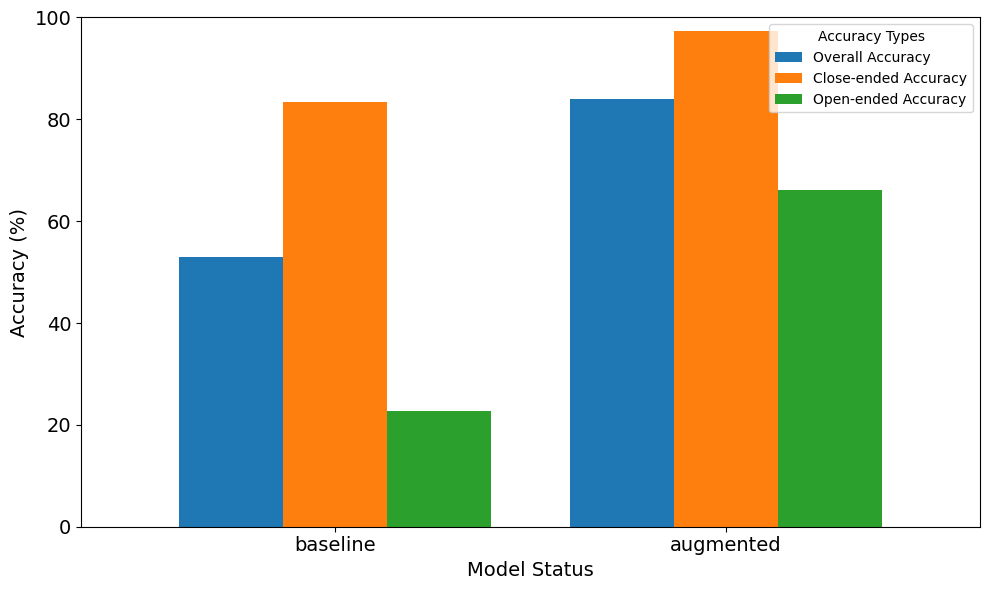
\includegraphics[width=\textwidth]{image/bab4/blip-pathvqa.png}
  \caption{Perbandingan akurasi model BLIP dengan \textit{dataset} PathVQA sebelum dan sesudah dilakukan augmentasi data pertanyaan}
  \label{fig:perbandingan-akurasi-blip-pathvqa}
\end{figure}

\par Lalu, untuk model BLIP yang dilatih dengan \textit{dataset} VQA-RAD juga menghasilkan performa yang lebih baik setelah dilakukan augmentasi data pertanyaan. Hal ini dapat dilihat dari peningkatan nilai akurasi, akurasi \textit{close-ended}, dan akurasi \textit{open-ended} dari \textit{baseline} model yang sebelumnya dilatih tanpa augmentasi data pertanyaan dengan konfigurasi \textit{hyperparameter} \textit{epochs} 15, \textit{batch size} 8, dan \textit{learning rate} $1 \times 10^{-5}$ menghasilkan akurasi 39,73\%, akurasi \textit{close-ended} 61,54\%, dan akurasi \textit{open-ended} 39,64\%. Pada \textit{dataset} VQA-RAD yang telah dilakukan augmentasi data pertanyaan, model BLIP menghasilkan akurasi 82,86\%, akurasi \textit{close-ended} 87,85\%, dan akurasi \textit{open-ended} 76,82\% dengan \textit{hyperparameter} \textit{epochs} 45, \textit{batch size} 8, dan \textit{learning rate} $5 \times 10^{-5}$. Hal ini menunjukkan bahwa nilai akurasi meningkat sebesar 43,13\%, dikarenakan akurasi \textit{close-ended} meningkat sebesar 26,31\% dan akurasi \textit{open-ended} yang juga meningkat sebesar 37,18\%. Pada Gambar \ref{fig:perbandingan-akurasi-blip-vqa-rad} menunjukkan perbandingan \textit{baseline} model dengan model BLIP setelah dilakukan augmentasi data pertanyaan.

\begin{figure}[H]
  \centering
  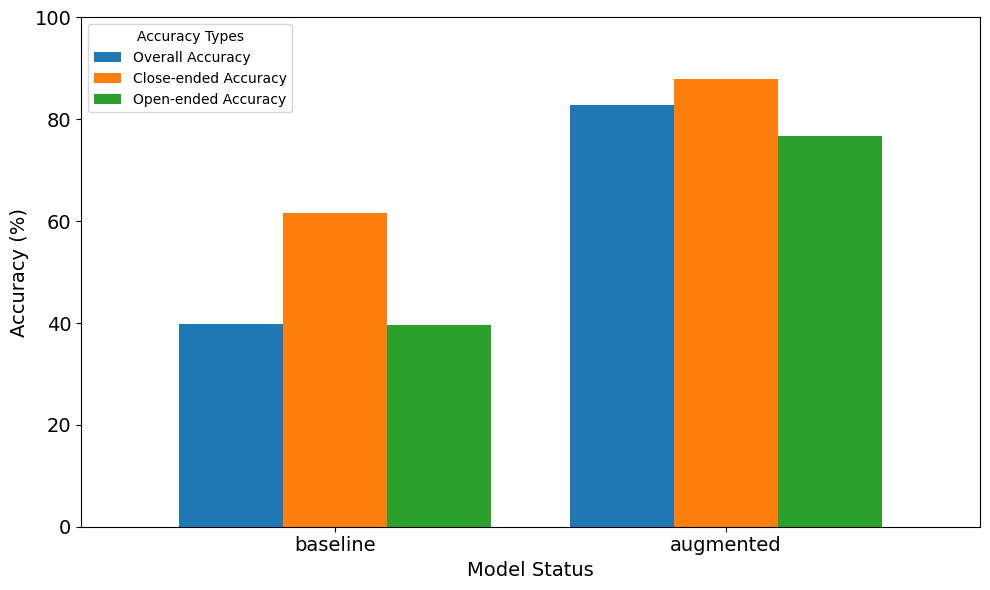
\includegraphics[width=\textwidth]{image/bab4/blip-vqarad.png}
  \caption{Perbandingan akurasi model BLIP dengan \textit{dataset} VQA-RAD sebelum dan sesudah dilakukan augmentasi data pertanyaan}
  \label{fig:perbandingan-akurasi-blip-vqa-rad}
\end{figure}

\par Sedangkan untuk model VGG19-LSTM yang dilatih dengan \textit{dataset} PathVQA tidak menghasilkan performa yang lebih baik setelah dilakukan augmentasi data pertanyaan. Hal ini karena hasil yang didapatkan tidak menunjukkan peningkatan nilai akurasi, akurasi \textit{close-ended}, dan akurasi \textit{open-ended} dari \textit{baseline} model yang sebelumnya dilatih tanpa augmentasi data pertanyaan dengan konfigurasi \textit{hyperparameter} \textit{epochs} 15, \textit{batch size} 8, dan \textit{learning rate} $1 \times 10^{-5}$ menghasilkan akurasi 26,96\%, akurasi \textit{close-ended} 43,73\%, dan akurasi \textit{open-ended} 10,16\%. Pada \textit{dataset} PathVQA yang telah dilakukan augmentasi data pertanyaan, model VGG19-LSTM menghasilkan akurasi 25,87\%, akurasi \textit{close-ended} 41,73\%, dan akurasi \textit{open-ended} 0,10\% dengan \textit{hyperparameter} \textit{epochs} 15, \textit{batch size} 8, dan \textit{learning rate} $1 \times 10^{-5}$. Hal ini menunjukkan bahwa adanya penurunan nilai akurasi sebesar 1,09\%, dikarenakan akurasi \textit{close-ended} yang mengalami penurunan sebesar 2,00\% dan akurasi \textit{open-ended} yang mengalami penurunan sebesar 10,06\%. Lalu, pada saat mengevaluasi dengan BLEU pada pertanyaan \textit{open-ended} menunjukkan bahwa kemampuan model VGG19-LSTM yang dilatih dengan \textit{dataset} PathVQA hampir tidak dapat dipahami dalam mengevaluasi jawaban untuk kata tunggal, pasangan dua kata yang berurutan, dan frasa tiga kata yang berurutan, dikarenakan nilai BLEU-1, BLEU-2, dan BLEU-3 yang didapat adalah 0,19, 0,06, dan 0,05. Pada Gambar \ref{fig:perbandingan-akurasi-vgg19-lstm-pathvqa} menunjukkan perbandingan \textit{baseline} model dengan model VGG19-LSTM setelah dilakukan augmentasi data pertanyaan.

\begin{figure}[H]
  \centering
  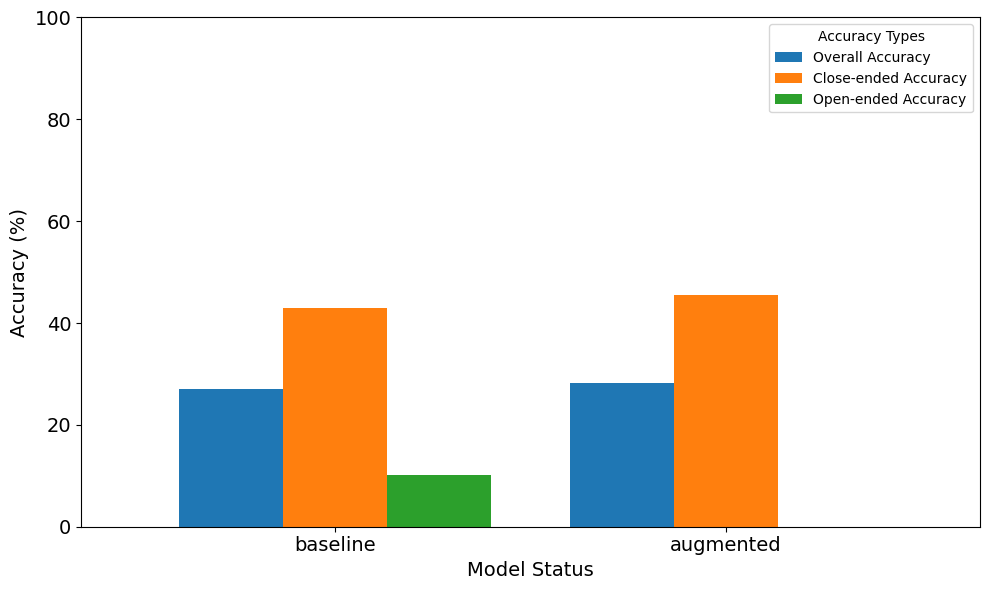
\includegraphics[width=\textwidth]{image/bab4/vgg19-lstm-pathvqa.png}
  \caption{Perbandingan akurasi model VGG19-LSTM dengan \textit{dataset} PathVQA sebelum dan sesudah dilakukan augmentasi data pertanyaan}
  \label{fig:perbandingan-akurasi-vgg19-lstm-pathvqa}
\end{figure}

\par Lalu, untuk model VGG19-LSTM yang dilatih dengan \textit{dataset} VQA-RAD menghasilkan performa yang baik setelah dilakukan augmentasi data pertanyaan. Walaupun hasil yang didapat tidak sebaik model BLIP, namun hasil yang didapat menunjukkan peningkatan performa setelah dilakukan augmentasi data pertanyaan. Hal ini dapat dilihat dari peningkatan nilai akurasi, akurasi \textit{close-ended}, dan akurasi \textit{open-ended} dari \textit{baseline} model yang sebelumnya dilatih tanpa augmentasi data pertanyaan dengan konfigurasi \textit{hyperparameter} \textit{epochs} 15, \textit{batch size} 8, dan \textit{learning rate} $1 \times 10^{-5}$ menghasilkan akurasi 24,44\%, akurasi \textit{close-ended} 43,52\%, dan akurasi \textit{open-ended} 6,84\%. Pada \textit{dataset} VQA-RAD yang telah dilakukan augmentasi data pertanyaan, model VGG19-LSTM menghasilkan akurasi 41,64\%, akurasi \textit{close-ended} 62,40\%, dan akurasi \textit{open-ended} 16,54\% dengan \textit{hyperparameter} \textit{epochs} 15, \textit{batch size} 8, dan \textit{learning rate} $1 \times 10^{-5}$. Hal ini menunjukkan bahwa nilai akurasi meningkat sebesar 17,20\%, dikarenakan akurasi \textit{close-ended} meningkat sebesar 18,88\% dan akurasi \textit{open-ended} yang juga meningkat sebesar 9,70\%. Ketika mengevaluasi dengan BLEU pada pertanyaan \textit{open-ended} menunjukkan bahwa kemampuan model VGG19-LSTM yang dilatih dengan \textit{dataset} VQA-RAD sulit untuk memahami kata tunggal dan dua kata yang berurutan, dikarenakan nilai BLEU-1 dan BLEU-2 yang didapat adalah 17,17 dan 10,5. Sementara itu, model VGG19-LSTM ini juga hampir tidak mampu memahami frasa tiga kata yang berurutan, hal ini dikarenakan nilai BLEU-3 yang tercatat sebesar 7,39. Pada Gambar \ref{fig:perbandingan-akurasi-vgg19-lstm-vqa-rad} menunjukkan perbandingan \textit{baseline} model dengan model VGG19-LSTM setelah dilakukan augmentasi data pertanyaan.

\begin{figure}[H]
  \centering
  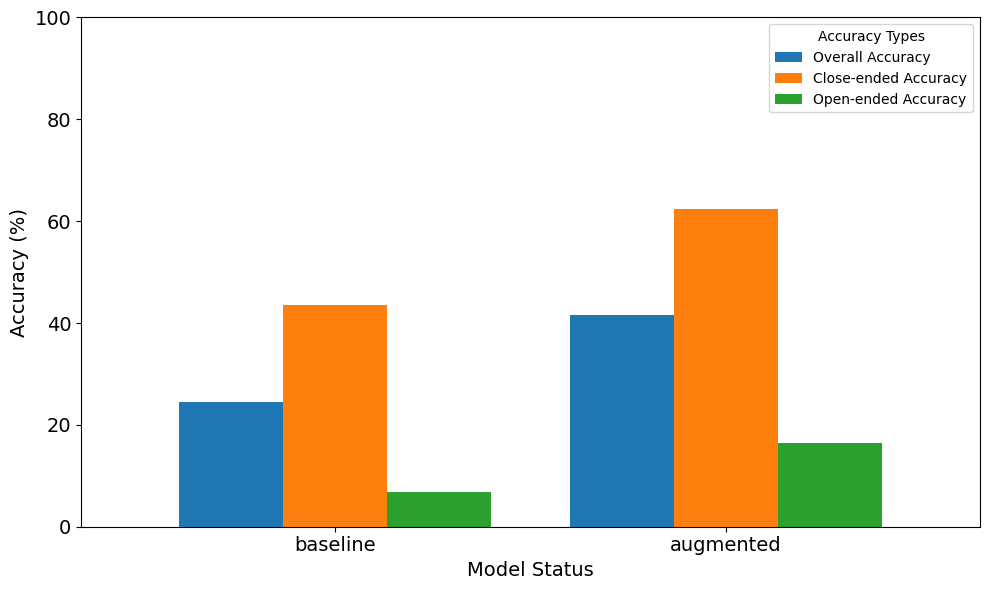
\includegraphics[width=\textwidth]{image/bab4/vgg19-lstm-vqarad.png}
  \caption{Perbandingan akurasi model VGG19-LSTM dengan \textit{dataset} VQA-RAD sebelum dan sesudah dilakukan augmentasi data pertanyaan}
  \label{fig:perbandingan-akurasi-vgg19-lstm-vqa-rad}
\end{figure}


\par Dari semua eksperimen yang sudah dilakukan, dapat dilihat bahwa nilai akurasi untuk pertanyaan \textit{close-ended} lebih tinggi dibandingkan dengan pertanyaan \textit{open-ended}. Hal ini bisa saja disebabkan dikarenakan pertanyaan \textit{close-ended} memiliki distribusi yang lebih banyak dibandingkan dengan pertanyaan \textit{open-ended}. Lalu, dapat disimpulkan juga bahwa model BLIP yang dilatih dengan \textit{dataset} PathVQA dan VQA-RAD menghasilkan performa yang lebih baik dibandingkan dengan model VGG19-LSTM. Hal ini menunjukkan bahwa model BLIP yang dilatih dengan \textit{dataset} PathVQA dan VQA-RAD dapat digunakan untuk menjawab pertanyaan berdasarkan citra patologi dan radiologi dengan performa yang lebih baik dibandingkan dengan model VGG19-LSTM.

\section{Pengembangan Sistem Medis Cerdas Berbasis Web}

\par Pada pengembangan sistem medis cerdas berbasis web ini meliputi tiga halaman, yaitu halaman utama, halaman untuk menjawab pertanyaan berdasarkan citra patologi, dan halaman untuk menjawab pertanyaan berdasarkan citra radiologi. Pada halaman utama, pengguna dapat memilih jenis citra yang diinginkan, yaitu citra patologi atau citra radiologi. Halaman utama ini dapat dilihat pada Gambar \ref{fig:halaman-utama}. Halaman utama ini akan mengarahkan pengguna ke halaman untuk menjawab pertanyaan berdasarkan citra patologi atau radiologi sesuai dengan pilihan pengguna.

\begin{figure}[H]
    \centering
    \label{fig:halaman-utama}
    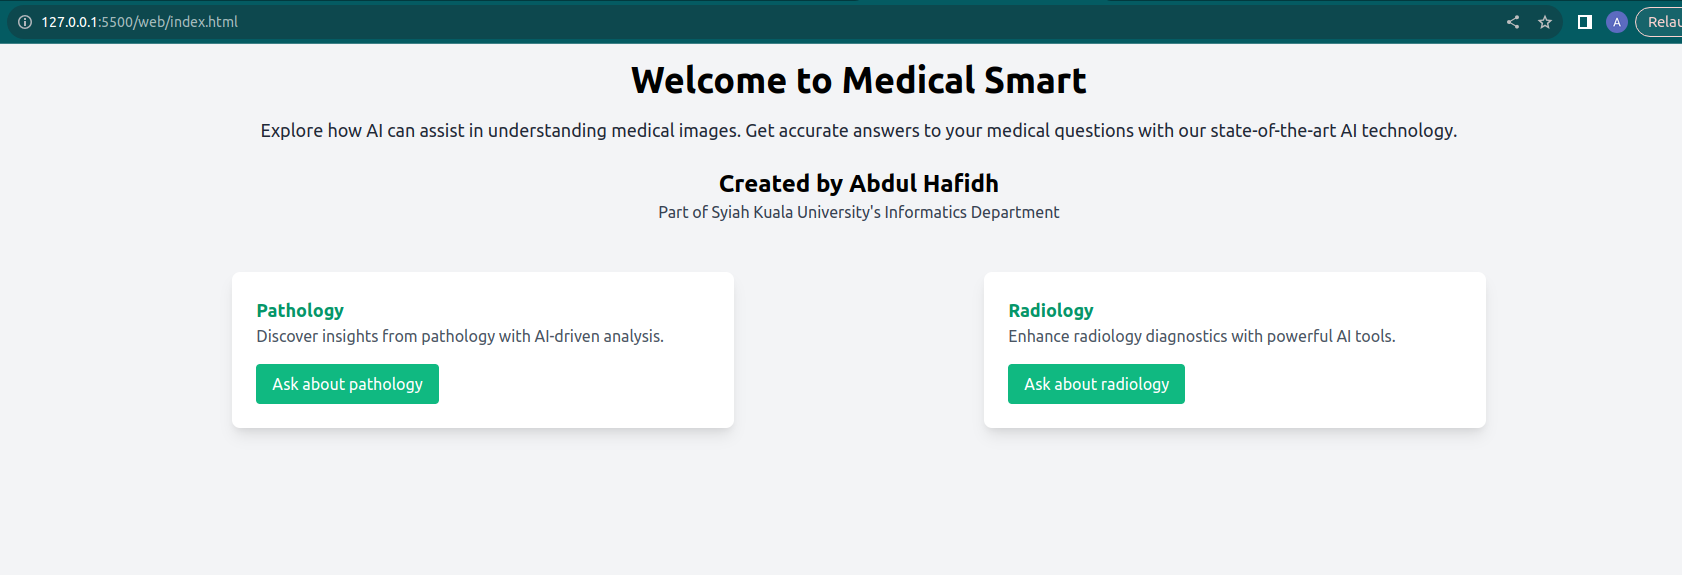
\includegraphics[width=\textwidth, height = 7cm]{image/bab4/halaman_utama.png}
    \caption{Halaman utama sistem medis cerdas berbasis web}
    \label{fig:halaman-utama}
\end{figure}

\par Pada halaman untuk menjawab pertanyaan berdasarkan citra patologi, pengguna dapat mengunggah citra patologi dan menuliskan pertanyaan yang ingin diajukan. Halaman ini akan menampilkan jawaban dari pertanyaan yang diajukan berdasarkan citra patologi yang diunggah. Halaman ini dapat dilihat pada Gambar \ref{fig:halaman-patologi}.

\begin{figure}[H]
  \centering
  \label{fig:halaman-patologi}
  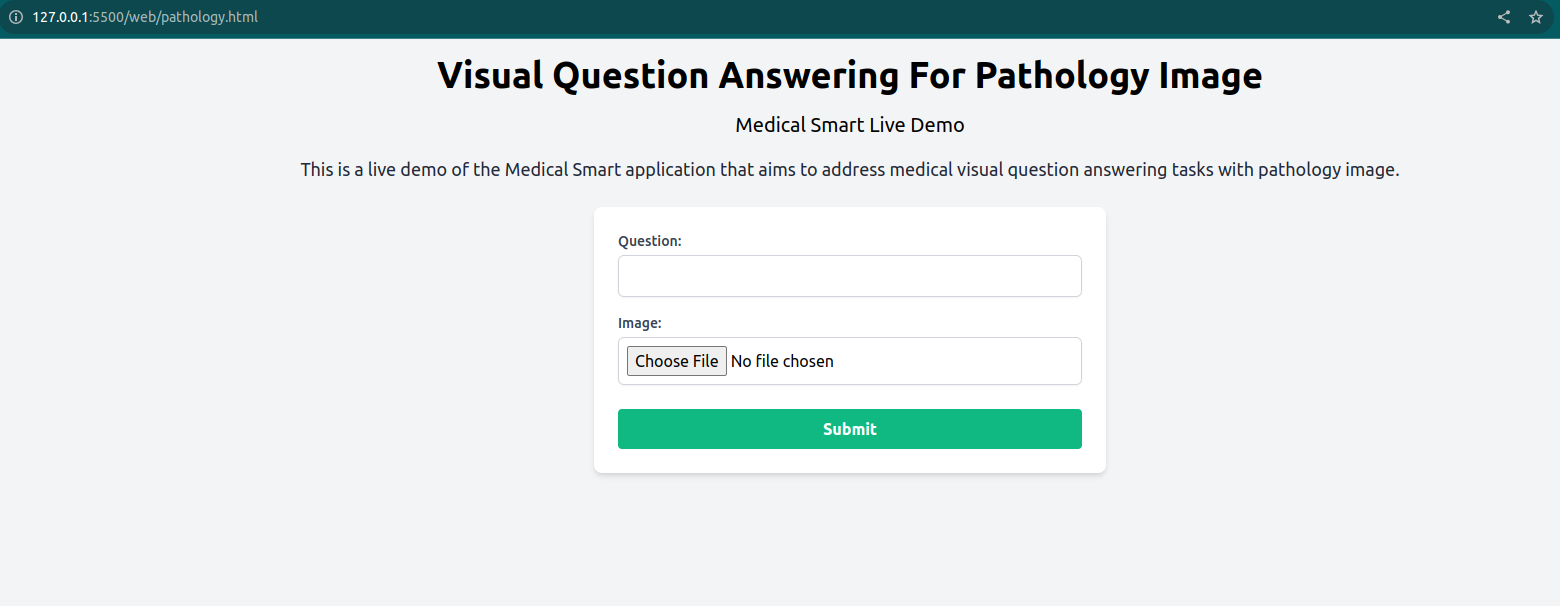
\includegraphics[width=\textwidth, height = 7cm]{image/bab4/halaman_patologi.png}
  \caption{Halaman untuk menjawab pertanyaan berdasarkan citra patologi}
  \label{fig:halaman-patologi}
\end{figure}

Pada halaman untuk menjawab pertanyaan berdasarkan citra radiologi, pengguna dapat mengunggah citra radiologi dan menuliskan pertanyaan yang ingin diajukan. Halaman ini akan menampilkan jawaban dari pertanyaan yang diajukan berdasarkan citra radiologi yang diunggah. Halaman ini dapat dilihat pada Gambar \ref{fig:halaman-radiologi}.

\begin{figure}[H]
  \centering
  \label{fig:halaman-radiologi}
  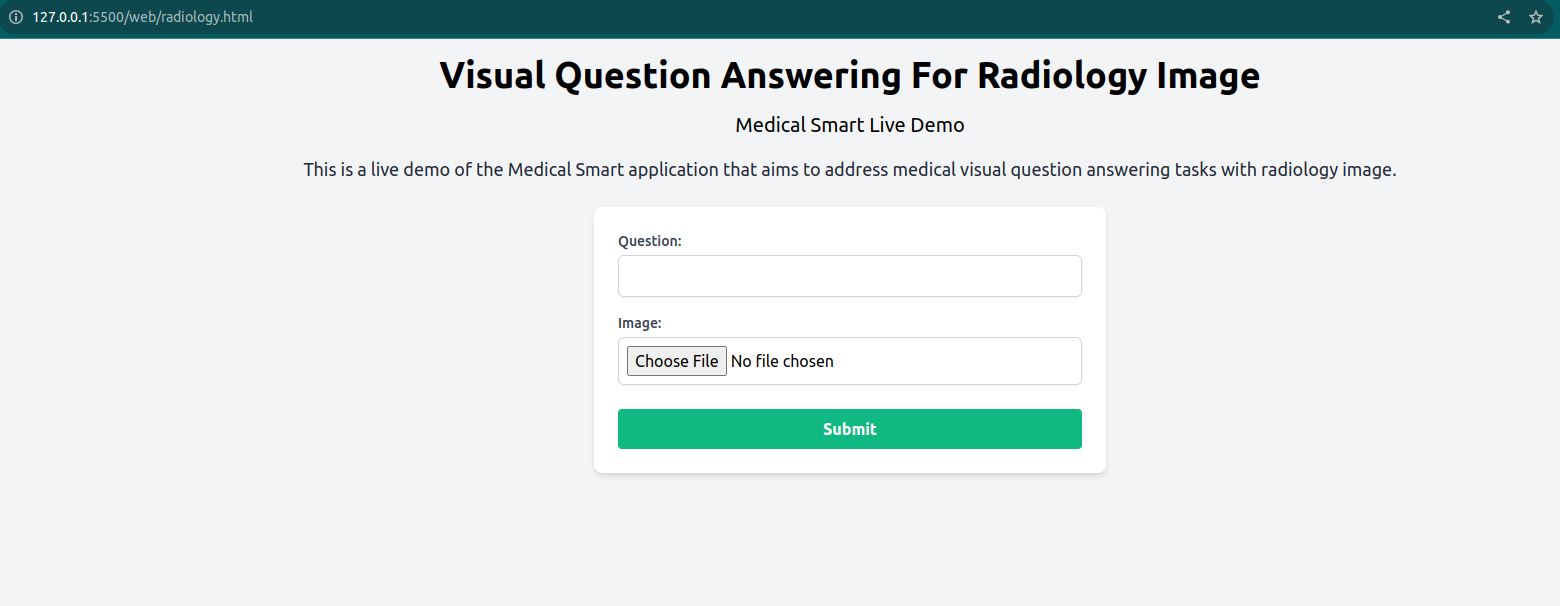
\includegraphics[width=\textwidth]{image/bab4/halaman_radiologi.png}
  \caption{Halaman untuk menjawab pertanyaan berdasarkan citra radiologi}
  \label{fig:halaman-radiologi}
\end{figure}

\par Model yang digunakan dalam sistem ini adalah model BLIP, dikarenakan model BLIP yang dilatih dengan \textit{dataset} PathVQA dan VQA-RAD yang telah dilakukan augmentasi data pertanyaan menghasilkan performa yang lebih baik dibandingkan dengan model VGG19-LSTM. Model BLIP yang dilatih dengan \textit{dataset} PathVQA yang telah dilakukan augmentasi data pertanyaan dengan \textit{hyperparameter} \textit{epochs} 15, \textit{batch size} 8, dan \textit{learning rate} $1 \times 10^{-5}$ akan digunakan untuk menjawab pertanyaan berdasarkan citra patologi. Model BLIP yang dilatih dengan \textit{dataset} VQA-RAD yang telah dilakukan augmentasi data pertanyaan dengan \textit{hyperparameter} \textit{epochs} 45, \textit{batch size} 8, dan \textit{learning rate} $5 \times 10^{-5}$ akan digunakan untuk menjawab pertanyaan berdasarkan citra radiologi.

\par Setelah memilih model yang akan digunakan, disini akan dilakukan tahap kuantisasi model yang bertujuan dalam memperkecil ukuran model tanpa mengorbankan performa dan mempercepat proses inferensi. Pada tahap kuantisasi model ini akan dilakukan dengan menggunakan metode \textit{dynamic quantization} yang disediakan oleh \textit{framework} PyTorch untuk tahapan kuantisasi ini. Pada Tabel \ref{tab:spesifikasi-model} menunjukkan spesifikasi model BLIP sebelum dan sesudah dikuantisasi pada \textit{dataset} PathVQA dan VQA-RAD untuk membandingkan ukuran model dan rata-rata waktu inferensi.

% Please add the following required packages to your document preamble:
% \usepackage{multirow}
\begin{table}[H]
  \centering
  \caption{Spesifikasi model BLIP sebelum dan sesudah dikuantisasi}
  \label{tab:spesifikasi-model}
  \begin{tabular}{|l|l|l|l|}
  \hline
  \textit{\textbf{Dataset}} & \textbf{Status} & \textbf{\begin{tabular}[c]{@{}l@{}}Ukuran \\ model\end{tabular}} & \textbf{\begin{tabular}[c]{@{}l@{}}Rata-rata\\ waktu inferensi\end{tabular}} \\ \hline
  \multirow{2}{*}{PathVQA} & Tidak dikuantisasi & 1467,73 MB & 0,24 detik \\ \cline{2-4} 
   & Sudah dikuantisasi & 508,21 MB & 0,20 detik \\ \hline
  \multirow{2}{*}{VQA-RAD} & Tidak dikuantisasi & 1467,73 MB & 0,21 detik \\ \cline{2-4} 
   & Sudah dikuantisasi & 508,20 MB & 0,17 detik \\ \hline
  \end{tabular}
\end{table}

\par Pada proses pengembangan \textit{backend} pada sistem ini menggunakan \textit{framework} FastAPI untuk dilakukan \textit{deploy} model yang telah dikuantisasi menjadi sebuah API. Disini dipilih model yang telah dikuantisasi karena ukuran model yang lebih kecil dan rata-rata waktu inferensi yang lebih cepat dibandingkan dengan model yang tidak dikuantisasi sesuai dengan Tabel \ref{tab:spesifikasi-model}. Tabel \ref{tab:daftar-endpoint} menunjukkan daftar API \textit{endpoint} pada sistem medis cerdas berbasis web yang digunakan untuk menjawab pertanyaan berdasarkan citra patologi dan radiologi.


% Please add the following required packages to your document preamble:
% \usepackage{multirow}
% \usepackage{graphicx}
\begin{table}[H]
  \centering
  \caption{Daftar API \textit{endpoint} pada sistem medis cerdas berbasis web}
  \label{tab:daftar-endpoint}
  \resizebox{\columnwidth}{!}{%
  \begin{tabular}{|r|l|l|l|}
  \hline
  \multicolumn{1}{|l|}{\textbf{No}} & \textit{\textbf{Method}} & \textit{\textbf{Endpoint}} & \textbf{Deskripsi} \\ \hline
  1 & \multirow{2}{*}{POST} & /predict/pathology & Menjawab pertanyaan berdasarkan citra patologi \\ \cline{1-1} \cline{3-4} 
  2 &  & /predict/radiology & Menjawab pertanyaan berdasarkan citra radiologi \\ \hline
  \end{tabular}%
  }
  \end{table}

  Tabel \ref{tab:daftar-endpoint} memaparkan daftar API \textit{endpoint} pada sistem medis cerdas berbasis web, yang dirancang untuk menjawab pertanyaan yang berkaitan dengan citra patologi dan radiologi. Kedua \textit{endpoint} ini diakses melalui \textit{method} "POST" dan menerima masukan berupa gambar serta pertanyaan yang diinginkan. Hasil yang diberikan adalah jawaban terhadap pertanyaan tersebut dalam format JSON.

  Dalam konteks sistem ini, ketika pengguna menekan tombol \textit{"Submit"} pada halaman yang ditujukan untuk pertanyaan berbasis citra patologi atau radiologi, akan terjadi \textit{request} ke API \textit{endpoint} yang relevan. Dalam hal ini, \textit{request} ini mengirimkan gambar bersama dengan pertanyaan yang akan dijawab. Setelah \textit{request} diterima oleh \textit{endpoint}, sistem akan melakukan inferensi menggunakan model yang telah dikuantisasi untuk memproses data tersebut. Hasil inferensi berupa lima jawaban yang mungkin benar akan disimpan dalam format JSON, kemudian hasil dari JSON akan dikirim ke halaman pengguna untuk ditampilkan. Pada saat yang sama, hasil jawaban akan diberi \textit{confidence score} yang menunjukkan tingkat keyakinan model terhadap jawaban yang diberikan. 

  \par Setelah pengembangan \textit{backend} selesai, maka proses percobaan untuk menjawab pertanyaan berdasarkan citra patologi dan radiologi dapat dilakukan. Pada uji coba dalam menjawab pertanyaan berdasarkan citra patologi dapat dilihat pada Lampiran 10, sedangkan pada uji coba dalam menjawab pertanyaan berdasarkan citra radiologi dapat dilihat pada Lampiran 11.
  




% Baris ini digunakan untuk membantu dalam melakukan sitasi
% Karena diapit dengan comment, maka baris ini akan diabaikan
% oleh compiler LaTeX.
\begin{comment}
\bibliography{daftar-pustaka}
\end{comment}